\chapauthor{Иванюк Д.С.\\Таберко В.В.\\Прохоренко В.А.\\Смородин В.С.}
\chapter{Автоматизация производственной деятельности в рамках Экосистемы OSTIS}
\chapauthortoc{Иванюк Д.С.\\Таберко В.В.\\Прохоренко В.А.\\Смородин В.С.}
\label{chapter_enterprise}

\abstract{Современные направления научно-технической деятельности в области оптимизации  функционирования производств требуют разработки актуальных подходов в реализации адаптивного управления производственной деятельностью с использованием элементов искусственного интеллекта, нейросетевого моделирования и разработки интеллектуальных компьютерных систем на основе использования новых технологий.

В настоящем разделе предлагается подход к построению интеллектуальной компьютерной системы адаптации управления нового поколения в рамках Экосистемы OSTIS. Формализация компьютерной системы адаптации управления реализуется на основе онтологии предметной области ``технологические процессы производства с вероятностными характеристиками'', реализованной посредством применения OSTIS-систем в рамках технологии OSTIS.

В основе создания гибридной интеллектуальной системы адаптации управления  лежит идея разработки математических моделей нейросетевых контроллеров, решающих задачи реализации методов и алгоритмов синтеза обратных связей по управлению технологическим циклом в зависимости от изменения параметров функционирования объекта управления в режиме реального времени, на основе использования средств программно-аппаратного сопряжения с технологическим циклом производства.}

Современное направление конвергенции работ в области создания интеллектуальных систем (см. \scncite{Golenkov2018}) требует разработки соответствующего программного обеспечения с элементами когнитивных способностей на основе семантически совместимых технологий искусственного интеллекта. Концепция Industry 4.0 предполагает построение единой онтологической модели предприятия (см. \scncite{Savushkin2018}), включающей в себя описание оборудования и технологических процессов производства. Технология OSTIS предоставляет средства для построения такой модели, обеспечивает возможность построения "цифрового двойника" предприятия на основе формализованного описания соответствующей предметной области. Полученная онтологическая модель, таким образом, может выступать основой интеграции востребованных интеллектуальных решений по автоматизации и информационному обеспечению производственной деятельности.

В первой части главы рассматривается подход к построению системы адаптивного управления технологическим процессом производства в виде решателя соответствующей ostis-системы на основе онтологии предметной области ``технологические процессы производства с вероятностными характеристиками''. В основу функционирования предлагаемой системы положено применение нейросетевых контроллеров. В основу формализации контура управления и математических моделей объекта исследования положены результаты научных разработок авторов в области имитационного моделирования сложных технических систем (\scncite{Smorodin2007}). Такая реализация позволяет обеспечить возможность интеграции предлагаемого решения с другими разработками, программными средствами предприятия для обеспечения построения интеллектуальных систем автоматизированного управления, рекомендательных систем и систем поддержки принятия решений, систем информационного обеспечения персонала предприятия.

Во второй части главы рассматриваются вопросы построения онтологической модели предприятия на примере предметной области "рецептурные производства" с применением общепринятых международных стандартов описания содержания производственной деятельности предприятия. Формализация стандартов является основой подхода к проектированию предприятия, в ее процессе требуется принять во внимание сложную специфику предметной области, возможность неоднозначной трактовки положений и необходимость обеспечения актуализации используемых стандартов. Онтологический подход к построению умных предприятий в рамках Экосистемы OSTIS показан на примере формализованного описания физической модели предприятия ОАО ``Савушкин продукт'' и построения системы автоматизации деятельности инженера-технолога.

\section{Адаптивное управление технологическим циклом производства на основе Технологии OSTIS}

В основу формализации контура управления и математических моделей объекта исследования положены результаты научных разработок авторов в области имитационного моделирования сложных технических систем (см. \scncite{Smorodin2007}).



\subsection{Онтология предметной области ``технологические процессы с вероятностными характеристиками''}

\subsubsection{Качественные характеристики технологических процессов}

Центральными понятиями в рассматриваемой предметной области являются технологический процесс (цикл) и вероятностный технологический процесс (\scncite{Smorodin2007}).

\begin{SCn}
    \scnheader{технологический процесс}
    \scnidtf{технологический цикл}
    \scnidtf{установленная  технологическими документами последовательность взаимосвязанных действий, направленных на объект процесса с целью получения требуемого конечного результата}
    \scnidtf{множество технологических операций  $\big\{TCO_{ij}\big\}$, где  $i,j= \overline{1,N}$, в совокупности с используемыми ими ресурсами }
\end{SCn}

В рамках стандарта ISA-88 в модели процедурного управления (procedural control module) это является процедурой (procedure), в результате выполнения которой появляется конечной партия продукта (возможно полуфабриката, который будет использоваться в дальнейшем для производства других партий продукции). 

\begin{SCn}
    \scnheader{вероятностный технологический процесс}
    \scnidtf{ВТП}
    \scnsubset{технологический процесс}
    \scnidtf{технологический процесс с вероятностными параметрами функционирования}
    \scnidtf{технологический процесс с изменяющейся в ходе его реализации структурой технологического цикла}
\end{SCn}

\begin{SCn}
	\scnheader{технологическая операция}
	\scnidtf{TCO}
	\scnsubset{технологический процесс}
	\scnidtf{часть технологического процесса, выполняемая непрерывно на одном рабочем месте над одним или несколькими одновременно обрабатываемыми или собираемыми изделиями, одним или несколькими исполнителями}
\end{SCn}

В рамках стандарта ISA-88 это является фазой (phase), в результате выполнения которой появляется несущественно изменяются свойства продукта. Шагами управлять оператор не может (стартовать/ставить на паузу/продолжать). Они могут выполняться последовательно, параллельно или в комбинации данных вариантов.


\begin{SCn}
	\scnheader{Микротехнологическая операция}
	\scnidtf{MTCO}
	\scnsubset{технологическая операция}
    \scnidtf{конечная последовательность элементарных операций, составляющих в совокупности содержание технологической операции,  выполняемой непрерывно на одном рабочем месте}
\end{SCn}



Традиционно рассматривают две группы технологических процессов:
\begin{textitemize}
	\item непрерывного типа
	\item дискретного типа
\end{textitemize}

Первая группа технологических процессов обычно реализуется на производстве в режиме реального времени. Данные технологические процессы являются объектом АСУТП. Примером применения АСУТП является контроль за процессом выплавки стали, контроль за поступлением сырья в мартеновские печи и автоматической разливкой металла по формам. Вторая группа технологических процессов характеризуется графовой структурой организации технологического цикла, который реализуется в результате взаимодействия множества технологических операций $\big\{TCO_i\big\}$. Некоторые $TCO_i$ могут состоять, в свою очередь, из множества микротехнологических операций $\big\{MTCO_{ij}\big\}$.
В зависимости от способа вхождения $\big\{MTCO_{ij}\big\}$  в состав $\big\{TCO_i\big\}$ различают следующие типы технологических процессов:

\begin{textitemize}
	\item одноуровневые, в которых $\big\{MTCO_{ij}\big\}$ могут выполняться параллельно-последовательно (в соответствии с графовой структурой связей между $MTCO_{ij}$ );
	\item иерархические, в которых основная технологическая ветвь разделяется на несколько дочерних, после чего происходит обратное слияние; при этом в составе $MTCO_{ij}$ любого уровня иерархии имеются операции "расщепления"{} технологических линий и операция "сбора"{} технологических линий;
    \item итеративные, в которых дочерние операции вложены в основные операции; при этом результаты выполнения операций на одном уровне вложенности используются для выполнения дочерних технологических ветвей.
\end{textitemize}

Моделирование всех типов технологических процессов осуществляется либо на основе критических, либо на основе средних значений расхода ресурсов. Наиболее сложными для моделирования считаются вероятностные технологические процессы второго и третьего типов.

При выполнении $MTCO_{ij}$ осуществляется расход ресурсов технологического цикла. В зависимости от характера расхода этих ресурсов выделяют две группы процессов:

\begin{textitemize}
    \item детерминированные (ДТП), у которых расход ресурсов предприятия осуществляется по средним или максимальным значениям;
    \item вероятностные (ВТП), у которых одна часть ресурсов используется детерминированным способом, задаваемым списками ресурсов и их количеств, а другая часть ресурсов предприятия используется вероятностным способом, задаваемым с помощью функций вероятностей распределения значений ресурсов, необходимых для выполнения  $MTCO_{ij}$.
\end{textitemize}


\subsubsection{Надежностные характеристики функционирования оборудования}

Одноуровневые ВТП используют для своего выполнения устройства оборудования, которые могут иметь различные характеристики надежности функционирования.
Надежностные характеристики оборудования являются вероятностными и характеризуются следующим образом: моменты отказа определяются функцией распределения вероятностей значений времени безотказной работы устройства оборудования $F( \tau _{NOw})$, по истечении которого происходит отказ выполнения функций устройством. Отказы могут быть простыми, и после интервала времени восстановления $(\tau _{ROw})$ его функционирование возобновляется. Некоторые отказы могут с вероятностью $( P_{f1})$ приводить к простой аварии, которая требует для своей ликвидации дополнительного времени $( \tau _{EM1w})$ и дополнительной стоимости $( c _{EM1w})$. В этом случае имеет место авария оборудования 1-го типа. С вероятностью $( P_{f2})$ после обычного отказа может происходить авария 2-го типа, которая требует для своей ликвидации некоторой последовательности специальных технологических операций. Каждая такая технологическая операция может требовать дополнительного времени ее ликвидации $( \tau _{liq})$ и дополнительной стоимости ее выполнения $( c_{liq})$. В итоге ликвидация аварии 2-го типа может приводить к задержке выполнения $MTCO_{ij}$ из-за отказа оборудования на величину, равную сумме этих времен $\sum\tau_{liq}$ , и росту стоимости выполнения $MTCO_{ij}$ также на величину суммы стоимости $\sum\tau_{liq}$. После ликвидации отказов аварий 1-го и 2-го типа происходит лишь задержка времени выполнения и увеличение стоимости ее выполнения, а технологический процесс продолжает функционировать с ухудшенными временными и стоимостными характеристиками его реализации.

Устройства оборудования обладают некоторым ресурсом выполнения своих функций, который постепенно уменьшается и зависит от времени активного использования устройства. Специалисты по надежности обычно оперируют понятием ``время наработки устройства на отказ'' $(T_{TTF})$. При достижении значения времени активного использования устройства этого порогового значения вероятность отказа резко возрастает, и поэтому на практике стремятся либо переключить устройство на резервное (с временем фактического использования устройства близком к нулю), либо выполнить профилактические работы с целью восстановления ресурса времени использования устройства.

Имеются также ТП, в которых появление аварии оборудования 3-го типа приводит к отказу функционирования всего ТП. Аварии третьего типа ликвидируются аналогично ликвидации аварии 2-го типа с использованием специального оборудования и специальных бригад исполнителей. Но нормальное функционирование ТП приостанавливается.

Таким образом, проектное моделирование ВТП в силу  вероятностного характера запросов ресурсов множеством $\big\{MTCO_{ij}\big\}$ и наличия отказов оборудования, природа которых также вероятностная, представляет собой сложную научную задачу.


\subsubsection{Параметры (переменные) управления технологическим циклом}

Некоторые $MTCO_{ij}$ в ВТП используют не только ресурсы, но могут выполнять ряд контрольных функций за изменением значений компонентов множества переменных управления ВТП ${U_s}$. При нормальном выполнении ВТП каждый компонент этого множества должен находиться в допустимых диапазонах между минимальным ${U_s^-}$ и максимальным значением ${U_s^+}$ $s$-го компонента множества переменных управления ${U_s}$. Причем, изменения значения $U_s$ может иметь вероятностную природу.
При выполнении другой группы $MTCO_{ij}$ значения переменных управления могут корректироваться таким образом, чтобы $U_s$ возвращалось в допустимые пределы $(U_s^- \leq U_s\leq U_s^+)$ . Третья группа $\big\{MTCO_{ij}\big\}$ корректирует значения компонентов ${U_s}$ . Некоторые $MTCO_{ij}$ используются только для индикации состояний оборудования и ВТП.

По способу использования управляющих переменных можно разделить $\big\{MTCO_{ij}\big\}$ на следующие группы:

\begin{textitemize}
    \item индикации состояний ТП (используют минимальное число ресурсов);
    \item исполнительные элементы (не контролируют и не меняют компоненты ${U_s}$);
    \item контролирующие выход $U_s$ за допустимые диапазоны;
    \item восстанавливающие значения компонентов $U_s$ в отведенные диапазоны их изменения.
\end{textitemize}

В составе ВТП контролирующие $MTCO_{ij}$ могут изменяться вероятностным образом: выход за допустимые пределы $( P_{thr})$ на величину $( \triangle U_s)$ , которая в ту или в другую сторону может изменяться также вероятностным образом.


\subsubsection{Математическая модель микротехнологической операции}

Состав ресурсов, которые может использовать каждая $MTCO_{ij}$ , включает десять типов:
\begin{enumerate}
    \item Устройство оборудования индивидуального пользования
    \item Устройство оборудования общего пользования
    \item Ресурс индивидуального пользования
    \item Ресурс общего пользования
    \item Индивидуальные исполнители
    \item Бригады исполнителей
    \item Материалы
    \item Комплектующие
    \item Стоимость выполнения операций
    \item Время  выполнения операций
\end{enumerate}

Устройства оборудования индивидуального использования ($DEVBIN_r$) могут использовать какой-либо состав операций  на время ее выполнения  $\tau_{ij}$ Состав устройств общим количеством   может задаваться либо  персонального списком, либо  $MTCO_{ij}$ требуется для ее выполнения только число таких устройств, которые свободны на момент запроса операций ресурсов первого типа ($r=1$)

$MTCO_{ij}$ может затребовать для своего выполнения устройство оборудования общего пользования ($n_2$) специальным списком. На устройствах общего пользования номера $r$ выделяет место для  $ij$-й операции размером $V_{r2}$ на время ее выполнения, которое после окончания операции свободно для выделения другой операции. $V_{r2}$ является случайной величиной. Допускается конкуренция  $\big\{MTCO_{ij}\big\}$ за устройства общего пользования и место на этих устройствах.

Первые два типа ресурсов, являясь устройствами оборудования, могут отказывать в функционировании при их использовании $MTCO_{ij}$.

$MTCO_{ij}$ может потребовать для своего выполнения ресурсы индивидуального пользования ($r=3$) общим количеством $n_3$ и ресурсы общего пользования  в количестве $n_4$ ($r=4$). Ресурсы ($r=3$) и  ($r=4$) могут задаваться либо списком, либо для случая, когда номер ресурса не имеет значения, используются первые свободные $n_3$ или $n_4$ ресурсов.
От ресурсов ($r=1$) и ($r=2$) эти ресурсы отличаются только тем, что это абсолютно надежные устройства, которые выделяются в распоряжение $MTCO_{ij}$ на время ее выполнения, а затем снова перераспределяются между $\big\{MTCO_{ij}\big\}$ , либо на принципах конкуренции их за эти ресурсы, либо специальным образом зарезервированными за операциями место на общем ресурсе ($r=4$) также может выделяться нескольким операциям  и величина запроса является случайной величиной, которая задается с помощью функции распределения $F_{6ij}(V_{r4})$.

Любая $MTCO_{ij}$ может требовать конкретное число исполнителей индивидуальных ($n_5$)  и бригад исполнителей ($n_6$) . Состав бригад определяется списком размера ($n_6$). Эти запросы являются детерминированными величинами.

Ресурсы 7-10 имеют вероятностную природу. В общем случае для выполнения операции  $MTCO_{ij}$ расходуется $k_1$-го типа материалы ($mt_{k1}$) и комплектующие $k_2$-го типа ($prt_{k2}$). Количества таких вероятностных ресурсов равны соответственно $n_{7k1}$ и $n_{8k2}$ и представляют собой детерминированные величины.
Расход количества материалов определяется с помощью функций распределения $F_{4k2ij}(mt)$ и расход количества комплектующих также задается с помощью соответствующих функций распределения $F_{3k2ij}(prt)$.

Для нормального выполнения операции $MTCO_{ij}$ требуется расход ресурсов $r=9$ и $r=10$ финансовых затрат и времени выполнения операции. Обе эти характеристики являются случайными величинами  и поэтому запросы этих ресурсов задаются соответственно с помощью функций вероятности распределения их значений $F_{2ij}(C)$  и $F_{1ij}( \tau )$.


\subsubsection{Модель функционирования устройств оборудования}

Устройства оборудования используются двух типов: индивидуального использования ($DEVIN_{r1}$) номера $r_1$  и общего пользования ($DEVSHR_{r2}$)  номера  $r_2$.  Для устройства $DEVSHR_{r2}$ имеется ограничение места, которые разные  $MTCO_{ij}$ могут одновременно использовать размером $V_{0r2}$, задаваемым в начале имитации. За каждый $MTCO_{ij}$ резервируется определенное место $V_{r2ij}$, при этом всегда проверяется, чтобы сумма используемых мест  на $DEVSHR_{r2}$ была бы меньше $V_{0r2}$. В противном случае формируется отказ $MTCO_{ij}$ в использовании $DEVSHR_{r2}$, что приводит к ожиданию появления места в случае завершения предыдущей $MTCO_{ij}$.

Устройства оборудования обоих типов могут отказывать в функционировании. При этом они имеют надежностные характеристики вероятностной природы. Для каждого времени нахождения устройства $r$  в состояниях задаются функции вероятностей распределения значений времени:
\begin{textitemize}
    \item безотказного функционирования $\Phi_{1r}(\tau_{NOr})$
    \item восстановление работоспособности после простого отказа $\Phi_{2r}(\tau_{ROr})$
    \item ликвидации аварии 1-го типа $\Phi_{3r}(\tau_{em1})$;
    \item ликвидации аварии 2-го типа $\Phi_{5r}(\tau_{em2})$

\end{textitemize}

При появлении аварий время  использования оборудования (а следовательно и выполнение операции) возрастает и определяется с помощью функций вероятностей распределения значений стоимости:
\begin{textitemize}
    \item ликвидации аварии 1-го типа $\Phi_{4r}(C{em1})$;
    \item ликвидации аварии 2-го типа $\Phi_{6r}(C{em2})$
\end{textitemize}

Задаются также при появлении отказов оборудования  вероятности возникновения:
\begin{textitemize}
    \item ликвидации аварии 1-го типа ($P_{em1}$);
    \item ликвидации аварии 2-го типа ($P_{em2}$)
\end{textitemize}

Таким образом, время выполнения на оборудовании $r$ номера операции $MTCO_{ij}$ равно $1-(P_{em1}+P_{em2}) = P_{5A}$.  Каждое $r$-е устройство оборудования обладает пороговым значением времени наработки $t_{optr}$.



\subsubsection{Математическая модель вероятностного технологического процесса}

При реализации последовательных вероятностных технологических процессов (ВТП1) только одна из $MTCO_{ij}$ выполняется в текущий момент времени. При этом она может использовать все ресурсы предприятия или же эти ресурсы заранее распределены между операциями до начала реализации ВТП1. Поэтому в последовательных ВТП используются только устройства индивидуального пользования. Кроме того, в ВТП1 имеется несколько нестандартных $MTCO_{ij}$:
\begin{textitemize}
    \item одиночного оперативного резервирования устройств оборудования в тех случаях, когда фактическое время наработки на отказ $t_{n1}$ приблизится к критическому значению времени наработки $T_{N_{crit}}$;
    \item групповое резервирование устройств оборудования, если время наработки на отказ достигает критической величины одновременно у группы устройств;
    \item проведение профилактического ремонта всех устройств оборудования, когда процент устройств, требующих резервирования очень высок и при этом допустима остановка выполнения ВТП1;
    \item ликвидации аварий на устройствах для тех случаев, когда режимы резервирования и профилактики не удается заблаговременно выполнить.
\end{textitemize}



\begin{SCn}
	\scnheader{cистема управления}
	\scnidtf{СУ}
	\scnidtf{строго определённый набор программно-аппаратных средств для управления подконтрольным объектом, обеспечивающий возможность сбора показаний о его состоянии и воздействий на его поведение для достижения заданных целей}
\end{SCn}


\begin{SCn}
	\scnheader{автоматизированная система управления технологическим процессом}
	\scnidtf{АСУТП}
	\scnsubset{cистема управления}
    \scnidtf{комплекс технических и программных средств, обеспечивающих работу технологического оборудования в автоматическом (или автоматизированном) режиме в соответствии с выбранным критерием управления}
\end{SCn}


Быстротекущий вероятностный технологический процесс (ВТП2) обычно выполняется с высокой скоростью. Поэтому имитационная модель не успевает вмешиваться в динамику его реализации. Для этой цели имеется система управления (СУ), которая с помощью специального оборудования управляет его функционированием. Здесь также используется только оборудование индивидуального использования. Но это оборудование может выходить из строя. Поэтому крайне важно обеспечить своевременное резервирование устройств оборудования для предотвращения отказов и аварий в ВТП2. Состав и структура СУ ВТП2 известны технологу до имитации, и обычно это логические схемы, имеющие графовую структуру.

Вероятностный технологический процесс с параллельно-последовательной организацией (ВТП3) обычно имеет довольно низкую скорость реализации. Кроме того, эксперту-технологу известна технологическая схема реализации ВТП3. Как правило, группы   выполняются одновременно, однако сохраняется последовательный характер выполнения каждой $MTCO_{ij}$. Это означает, что внутри технологической схемы ВТП3 имеются устройства синхронизации типа ``И'', которые срабатывают по последнему во времени приходу сигналов активизации, после завершения предыдущих $MTCO_{ij}$. Эти сигналы имеют сложную структуру за счет их информационной "подкраски"{} признаками $\pi_{emij}$ (наличие аварии на оборудовании при выполнении  $MTCO_{ij}$) и $\pi_{uij}$ (наличие выхода компонентов вектора управления ${U_k}$ за допустимые пределы). После прихода последнего во времени сигнала на схему совпадения ``И'' на выходе формируется множество сигналов, активизирующих другую группу $\{MTCO_{ij}\}$ . Реализация ВТП3 начинается с первой $MTCO_{11}$ и завершается последней схемой совпадения ``И''. Все схемы синхронизации пронумерованы от $1$ до $n$, а $MTCO_{ij}$ имеет двойную нумерацию ( $i$ номер предыдущей схемы синхронизации, а $j$ номер последующей схемы синхронизации). Число входов и выходов у схем синхронизации может быть любым. Структура ВТП3 определяется графом связи $MTCO_{ij}$ , который задается с помощью таблицы коммутации операций в ВТП3.

В общем случае ВТП3 может использовать все ресурсы и оборудование в режиме конкуренции. Поэтому некоторые $MTCO_{ij}$ могут ожидать освобождения оборудования, а затем начинается имитация их выполнения. Связь между $MTCO_{ij}$ и собственно устройствами ВТП3 может осуществляться либо через специально выделенное оборудование индивидуального пользования, либо через любое из устройств оборудования, выделяемого $MTCO_{ij}$ на основе конкуренции. . Важной особенностью ВТП3 является возможность регулирования технологического процесса с помощью контроля за содержимым управляющих переменных и модификации значений компонентов вектора переменных управления $\{U_k\}$ с целью возврата их в отведенные для них диапазоны значений. Выполнение этой коррекции осуществляется специальными резервными $MTCO_{ij}$, регулирующими значения $\{U_k\}$ . Кроме того, ведется контроль за надежностью выполнения оборудованием своих функций. После ликвидации аварий оборудования в технологической цепи предусмотрены резервные $MTCO_{ij}$, которые ликвидируют последствия аварий на оборудовании. Наличие аварий оборудования и задержка активизации $MTCO_{ij}$ из-за нехватки ресурсов приводит к общему увеличению времени и стоимости выполнения всего множества {$MTCO_{ij}$}. Поэтому важным откликом ИМ ВТП3 является время выполнения {$MTCO_{ij}$} за один цикл имитации.

Параметрами моделирования являются начальное значение количества ресурсов, предоставленное в распоряжение всех $MTCO_{ij}$, и количество устройств оборудования, с помощью которых реализуется технологический цикл. Откликами ИМ ВТП3 являются суммарные расходы ресурсов вероятностного типа на один цикл имитации, а также коэффициенты использования ресурсов ВТП3 {$\eta_{r}$}. Статистиками имитации являются вектора значений удельных весов времени свершения событий в технологической схеме ВТП3.

Если ВТП3 является циклическим, то важными статистиками становятся среднее время цикла выполнения всего множества {$MTCO_{ij}$} до завершения имитации функционирования ВТП3 и минимально допустимый состав ресурсов и оборудования, при котором возможна его реализация.


%\subsubsection{Математическая модель системы управления вероятностным технологическим процессом}
%
%текст

\subsubsection{Имитационное моделирование технологических процессов}

Состав и функции операторов алгоритма имитации $MTCO_{ij}$ включают в себя:
\begin{enumerate}
    \item Начало активизации имитации операции - Интервал времени - $A_0$, Время - $t_{aij}$
    \item Формирование заказа ресурсов - Интервал времени - $A_1$, Время - $t_{1ij}$
    \item Захват свободных ресурсов на время выполнения операций - Интервал времени - $A_2$, Время - $t_{2ij}$
    \item Ожидание выделения освободившегося ресурса - $\tau_{wij}$ - Интервал времени - $A_3$
    \item Захват освободившегося ресурса - Интервал времени - $A_4$, Время - $t_{3ij}$
    \item Ожидание следующего освободившегося ресурса - $\tau_{w2ij}$ - Интервал времени - $A_5$
    \item Захват последнего из затребованных устройств на время выполнения - Интервал времени - $A_6$, Время - $t_{4ij}$
    \item Выполнение имитации операции - $\tau_{r2ij}$ - Интервал времени - $A_7$
    \item Конец выполнения операции, возврат захваченных ресурсов - Интервал времени - $A_8$, Время - $t_{5ij}$
    \item Формирование информации о характере использования оборудования - Интервал времени - $A_9$, Время - $t_{9ij}$
    \item Формирование информации о модификации значений компоненты вектора управления {$U_k$} - Интервал времени - $A_10$, Время - $t_{7ij}$
    \item Формирование адресата продолжения операции - Интервал времени - $A_11$, Время - $t_{8ij}$
\end{enumerate}

Надежностные характеристики функционирования устройств оборудования включают в себя:
\begin{enumerate}
    \item Время безотказного функционирования - с распределением $\Phi_{1r}(\tau_{NOr})$
    \item Время восстановления работоспособности  - с распределением $\Phi_{2r}(\tau_{RO})$
    \item Вероятность появления аварии 1-го типа - с вероятностью $P_{em1}$
    \item Время ликвидации аварии 1-го типа - с распределением $\Phi_{3r}(\tau_{em1})$
    \item Стоимость ликвидации аварии 1-го типа - с распределением $\Phi_{4r}(C_{em1})$
    \item Вероятность появления аварии 2-го типа - с вероятностью $P_{em2}$
    \item Время ликвидации аварии 2-го типа - с распределением $\Phi_{5r}(\tau_{em2})$
    \item Стоимость ликвидации аварии 2-го типа - с распределением $\Phi_{6r}(C_{em2})$
    \item Время наработки устройства на отказ - $T_{optr}$
\end{enumerate}

Состав и структура операторов алгоритма имитации функционирования устройств оборудования индивидуального пользования включает в себя:
\begin{enumerate}
    \item Начало активизации устройства $r$ - оператор $B_0$ - Момент времени - $t_{ar}$
    \item Розыгрыш по функции распределения $\tau_{NOK}$ - оператор $B_1$ - Момент времени -$t_{ar}$
    \item Определение типа использования оборудования - оператор $B_2$ - Момент времени -$t_{1r}$
    \item Имитация нормального использования устройства длительностью - Интервал времени - $\tau_{ij}$ - оператор $B_3$ $\tau_{ij}$ - Момент времени -$t_{1r}$
    \item Формирование признака  $\pi_{\Phi}:=0$ - оператор  $B_4$ - Момент времени - $t_{1r}$
    \item Активизация операции $ij$ - оператор $B_5$ - Момент времени - $t_{1r}$
    \item Розыгрыш по функции распределения $\tau_{ROK}$ - оператор $B_6$  - Момент времени -$t_{1r}$
    \item Имитация восстановления работоспособности устройств - оператор $B_7$ - Интервал времени - $\tau_{ROr}$
    \item Розыгрыш по $P_{em1}$ ситуации появления аварии 1-го типа - оператор $B_8$ - Момент времени -$t_{2r}$
    \item Имитация повторения имитации - оператор $B_9$ - Интервал времени - $\tau_{ij}$
    \item Формирование признака $\pi_{emk}:=0 $ - оператор $B_{10}$  - Момент времени -$t_{3r}$
    \item Розыгрыш по $P_{em2}$ ситуации появления аварии 2-го типа - оператор $B_{11}$ - Момент времени -$t_{2r}$
    \item Розыгрыш по функции распределения - Интервал времени - $\tau_{em1}$ - оператор $B_{13}$
    \item Имитация ликвидации аварии 1-го типа - оператор $B_{14}$ - Интервал времени - $\tau_{em1}$
    \item Имитация повторения операции - оператор $B_{15}$ - Интервал времени - $\tau_{ij}$
    \item Формирование признака $\pi_{emk}:=1$ и активизация операции - оператор $B_{16}$ - Момент времени -$t_{4r}$
    \item Розыгрыш по функции $P_{AV}$ ситуации появления аварии 2-го типа - оператор $B_{17}$ - Момент времени -$t_{2r}$
    \item Активизации последовательности процедур ликвидации сложной аварии и останов - оператор $B_{18}$ - Момент времени -$t_{2r}$
    \item Ожидание завершения ликвидации аварии 2-го типа - оператор $B_{19}$ - Интервал времени - $\tau_{w2r}$
    \item Формирование признака $\pi_{emk}:=1$ и активизация операции - оператор $B_{20}$ - Момент времени - $t_{5r}$
\end{enumerate}

Состав и функции операторов алгоритма имитации функционирования устройств общего пользования включают в себя:
\begin{enumerate}
    \item Активизация устройства - оператор - $C_0$ - Момент времени - $t_{ar}$
    \item Определение типа использования устройства - оператор - $C_1$ - Момент времени - $t_{ar}$
    \item Имитация нормального использования длительностью  $C_2$ - Интервал времени - $\tau_{ij}$
    \item Формирование признака $\pi_{ak}:=0$ и переход  - оператор - $C_3$ - Момент времени - $t_{1r}$
    \item Розыгрыш по функции распределения $\tau_{ROk}$ - оператор - $C_4$ - Момент времени - $t_{ar}$
    \item Имитация восстановления работоспособности устройств - оператор - $C_5$ - Интервал времени - $\tau_{ROk}$ - Момент времени - $t_{2r}$
    \item Розыгрыш по $P_{em1}$ ситуации появления аварии 1-го типа - оператор - $C_6$ - Момент времени - $t_{2r}$
    \item Имитация появления аварии  - оператор - $C_7$ - Интервал времени - $\tau_{ij}$
    \item Формирование признака $\pi_{ak}:=0$ и переход на $C_{19}$ - оператор - $C_8$ - Момент времени - $t_{3r}$
    \item Розыгрыш по $P_{em2}$ ситуации появления аварии 2-го типа - оператор - $C_{9}$ - Момент времени - $t_{3r}$
    \item Розыгрыш по функции распределения $\tau_{em2}$ - оператор - $C_{10}$  - Момент времени - $t_{3r}$
    \item Имитация ликвидации аварии 2-го типа $C_{11}$ - Интервал времени - $\tau_{em2}$
    \item Формирование признака $\pi_{emk}:=1$ и переход на $C_{19}$  - оператор - $C_{13}$  - Интервал времени - $\tau_{ij}$
    \item Розыгрыш по $P_{em2}$ ситуации появления аварии 2-го типа  - оператор -  $C_{15}$ - Момент времени - $t_{2r}$
    \item Активизация последовательности процедур ликвидации сложной аварии и останов $C_{16}$ - Момент времени - $t_{2r}$
    \item Ожидание завершения ликвидации аварии 2-го типа - оператор - $C_{17}$ - Интервал времени - $\tau_{w2k}$
    \item Формирование признака  $\pi_{emr}:=1$ - оператор - $C_{18}$  - Момент времени - $t_{5r}$
    \item Розыгрыш по функции распределения  $\tau_{NOk}$ нового значения интервала безотказного функционирования - оператор - $C_{19}$ - Момент времени - $t_{5r}$
    \item Активизация операции  - оператор - $C_{20}$ - Момент времени -  $t_{5r}$
\end{enumerate}


Таким образом описывается состав и функции операторов алгоритма имитации $MTCO_{ij}$ . В момент активизации  $MTCO_{ij}$ ($t_{aij}$)   выполняется оператор "начало активизации имитации" операции  ($A_0$).
С помощью оператора $A_1$ формируется заказ ресурсов для имитации выполнения  $MTCO_{ij}$.  Для этой цели используются функции распределения вероятностей их значений, приведенные в таблице 1.1.  В итоге выполнения оператора   формируется вектор детерминированных запросов ресурсов
\begin{equation*}
		(n_1,n_2,n_3,n_4,n_5,n_6,n_{7k1},n_{8k2})
\end{equation*}
и подмножество конкретных значений вероятностных характеристик запроса ресурса
\begin{equation*}
        ( \{V_{r2l}\} , \{V_{r4l}\} ; \{mt_{k1}\} , \{ko{k2}\} , c_{ijl} ;\tau_{ijl} )
\end{equation*}

Далее с помощью оператора захвата ресурсов $A_2$  на время выполнения операции осуществляется резервирование ресурсов, представленных множествами (1.1) и (1.2). В некоторых случаях из-за конкуренции $MTCO_{ij}$ за ресурсы может не оказаться свободных ресурсов или же места на ресурсах или устройствах. В этом случае с помощью оператора $A_3$  осуществляется ожидание освобождения ресурса длительностью $\tau_{w1ij}$. По мере освобождения ресурсов осуществляется захват частично освободившихся ресурсов с помощью оператора $A_4$ . Далее с помощью оператора $A_5$ операция $MTCO_{ij}$ ожидает освобождения следующего ресурса длительностью $\tau_{w2ij}$.  С помощью оператора $A_6$ имитируется захват последнего из затребованных ресурсов. И в момент $t_{4ij}$  начинается с помощью оператора $A_7$ имитация выполнения операции. Имитируется запуск всех устройств оборудования на заказанное время выполнения операции $\tau_{lij}$ сформированное с помощью функции распределения $F_{1ij}(\tau)$ . Имитация выполнения операции продолжается до тех пор, пока все устройства оборудования не завершат имитацию выполнения операции. Из-за отказов устройств оборудования и ликвидации аварий  оборудования фактическое время имитации операций может быть больше, чем заказанное время имитации $\tau_{zlij} \geq \tau_{ij}$.

С помощью оператора $A_7$ в момент времени $t_aij$ по окончании имитации операции все захваченные $MTCO_{ij}$ ресурсы возвращаются системе. В этот момент возможно продолжение тех $MTCO_{ij}$ , которые ждут освобождения ресурсов. По информации, поступившей от устройств оборудования о том, что имела место авария оборудования на хотя бы одном из устройств, формируется признак аварии ($\pi_{em}:=1$) оператором $A_9$.

С помощью оператора $A_{10}$ формируется признак модификации значений компонентов вектора переменных управления за допустимые пределы (т.е. $U_k \prec U_k^-$ или $U_k \succ  U_k^+$)  $\pi_{u}:=1$ ,	 в случае если $MTCO_{ij}$ является операцией  изменения $\{U_k\}$ . Для случая, когда $MTCO_{ij}$ является резервной операцией возврата переменных управления в допустимые пределы с помощью оператора $A_{10}$ осуществляется обратная модификация $\{U_k\}$ таким образом, чтобы $U_k^-  \leq  U_k  \leq U_k^+$   в момент времени $t_7ij$ . Наконец, с помощью оператора $A_{11}$ формируется адресат продолжения операции. При этом формируется сигнал сложного вида (информационно "подкрашенный"{} значениями признаков $\pi_{aij}$ и $\pi_{uij}$), которые согласно таблице коммутации $MTCO_{ij}$ в составе технологической схемы ВТП посылается на одно из устройств синхронизации типа ``ИЛИ'' и ``И''.  Эти устройства имеют нумерацию входов и поэтому в  адресате продолжения операции внутри сигнала указывается номер и номер входа устройства синхронизации.

Возможны четыре случая имитации операции на оборудовании:
\begin{textitemize}
    \item нормальное выполнение операции на всем оборудовании длительностью $\tau_{lij}$;
    \item имеет место восстановление функций оборудования хотя бы на одном из устройств $\tau_{2ij}>\tau_{lij}$;
    \item имела место авария 1-го типа на одном из устройств оборудования $\tau_{3ij}>\tau_{2ij}>\tau_{lij}$ ;
    \item имела место авария 2-го типа на любом из устройств оборудования  $\tau_{4ij}>\tau_{3ij}>\tau_{2ij}>\tau_{lij}$.
\end{textitemize}

Таким образом, наличие отказов и аварий устройств оборудования, а также ожиданий освобождения ресурсов в ряде случаев может существенно увеличить время выполнения операций по сравнению с разыгранным по функции распределения $F_{1ij}(\tau)$ с помощью жребия 3-го типа.

Это означает, что аварии оборудования приводят только к увеличению времени и стоимости выполнения $MTCO_{ij}$ и, как следствие, к росту общего времени и стоимости выполнения ВТП.

%!!!

%1.8.2- Имитационное моделирование функционирования устройств оборудования

В процессе имитации функционирования устройства оборудования фиксируется статистика фактического времени наработки устройства по формуле
\begin{equation*}
		t_{optr}:=t_{optr}+\tau_{ij}
\end{equation*}

При достижении $t_{optr}$ пороговой величины $T_{opt}$ вероятностиь отказа устройства настолько возрастает, что при следующем использовании устройства $r$ возможен отказ функционирования устройства, который может приведсти к появлению аварий на устройстве $r$ во время выполнения очередной операции $MTCO_{ij}$.

Одним из способов предотвращения ситуации может служить либо переключение на резервные устройства, либо проведение профилактики. После проведения одной из этих операций фактическое время наработки устройства устанавливается в нуль $t_{optr}:=0$ . Пороговое значение времени наработки указывается надежностных характеристиках для каждого $r$-го устройства оборудования.

В момент активации устройства номера $r$ операцией $MTCO_{ij}$ ($t_{ar}$) с помощью оператора $B_0$ осуществляется запись в базу данных конкретного номера устройства оборудования индивидуального пользования. Используя таблицу 1.3, с помощью функции распределения $\Phi_{1r}(\tau_{NOr})$  разыгрывается конкретное значение интервала безотказного функционирования устройства $\tau_{lrNOK}$.

Далее с помощью оператора $B_2$ в момент $t_{2r}$ определяется тип использования оборудования. Если выполняется неравенство $\tau_{lij}  \leq  \tau_{lrNOK}$ , то это означает нормальное использование устройства оборудования (без отказов). В подобном случае с помощью оператора $B_4$ формируется признак $\tau_{emr}:=0$, означающий отсутствие аварий.

С помощью оператора $B_5$ активизируется $MTCO_{ij}$, и имитация выполнения завершается с передачей информационного сигнала с признаком наличия аварии  ($\pi_{emr}:=0$).

Если же $\tau_{lij} \geq \tau_{lrNOr} $, то это означает случай 2 (наличие отказа оборудования). В этом случае с помощью оператора $B_6$ в момент $t_2$ по функции распределения $\Phi_{2r}(\tau_{ROr})$ формируется значение интервала восстановления работоспособности $\tau_{RORl}$. Затем осуществляется имитация восстановления работоспособности $r$-го устройства с помощью оператора $B_7$.  По завершении этой имитации по вероятности $P_{em1r}$ с помощью жребия 1-го типа моделируется появление аварии с помощью оператора $B_8$ в момент $( t_{2r} > \tau_{ROr} )$.  Далее операция повторяется с помощью оператора $B_{9}$ , который имитирует ее выполнение длительностью  $\tau_lij$. Эта ситуации означает отсутствие аварий, поэтому с помощью оператора $B_{10}$ формируется признак $\pi_{em}:=0$ . Далее с помощью оператора $B_11$ по вероятности $P_{em1}$ разыгрывается ситуация появления аварии 1-го типа. Разыгрывается по функции распределения длительности ликвидации аварий с помощью оператора $B_{13}$ и осуществляется имитация ликвидации аварий 1-го типа  длительностью $\tau_{lem1}$ оператором $B_14$. Далее аналогично имитируется повторение операции длительностью $\tau_{lij}$ с помощью оператора  $B_{19}$.  По завершении этой имитации оператор $B_{16}$ формирует признак ``была авария'' $\pi_{emr2}:=1$ и активизирует операцию  $MTCO_{ij}$. В противном случае с помощью оператора  $B_{17}$ в момент $t_{2r}$ по вероятности  $P_{a2}$ с помощью жребия 1-го типа формируется ситуация ``наличие аварии'' 2-го типа. С помощью оператора $B_18$ активизируется начальный элемент последовательности процедур ликвидации сложной аварии. Само же устройство $r_1$ останавливается и с помощью оператора $B_20$ имитируется ожидание завершения ликвидации аварии 2-го типа длительностью $\tau_{w2r}$.  Далее с помощью оператора $B_{20}$ активизируется устройство оборудования типа $2$. Устанавливается признак $\pi_{emr}:=1$  , активизируется операция $MTCO_{ij}$ и устройство останавливается, завершая имитацию  выполнения операции на устройстве в момент $t_{5r}$.

Может иметь место 4 случая:
\begin{textitemize}
    \item нормальное выполнение операции длительностью $( \tau_{ \phi 1 ij} = \tau_{ij} )$ ;

    \item автоматическое восстановление отказа без аварии на устройстве оборудования $r_1$ длительностью $( \tau_{\phi 2 ij} > \tau_{ij} )$ ;

    \item ликвидация аварии 1-го типа длительностью $( \tau_{\phi 3 ij} > \tau_{\phi 2 ij} > \tau_{ij} )$  ;

    \item наличие имитации аварии на оборудовании $r_1$ длительностью $( \tau_{ \phi 4 ij} \gg  \tau_{ij} )$ .

\end{textitemize}

Оборудование общего пользования имитируется по более сложному алгоритму. Надежностные характеристики устройств оборудования общего использования задаются аналогичным образом.

Основное отличие состоит в том, что в моменты завершения интервалы безотказного функционирования начинаются с начала имитации, поскольку это устройство функционирует непрерывно. Здесь также могут быть четыре случая:
\begin{textitemize}
    \item нормальное выполнение длительностью $\tau_{ij}$;
    \item наличие восстанавливаемого отказа длительностью  $(\tau_{ROlr2} + 2 \tau_{ij})$;
    \item ликвидация аварии 1-го типа длительностью  $(\tau_{ROlr2} + \tau_{em1r2} + 2 \tau_{ij})$;
    \item ликвидация аварии 2-го типа длительностью $(\tau_{ROlr2} + \tau_{O2r} + 2 \tau_{ij})$.
\end{textitemize}


Фактическое время выполнения операции возрастает с ростом сложности отказа оборудования. Сам же алгоритм имитации функционирования устройств общего пользования похож на алгоритм имитации функционирования устройств оборудования индивидуального пользования.



%1.8.3- Имитационное моделирование последовательного вероятностного технологического процесса

Вероятностный переход от одной к другой $MTCO_{ij}$ осуществляет элемент выбора операции. При этом он проверяет наличие критической ситуации устройств оборудования и своевременно активизирует нестандартные $MTCO_{ij}$.  После ликвидации нестандартной ситуации у устройств оборудования осуществляется переход на выполнение стандартных $MTCO_{ij}$ согласно матрице вероятностей перехода $\parallel P_{ij} \parallel $, где $i$ - номер предыдущей, а $j$ - номер последующей $MTCO_{ij}$.  Очевидно, что элемент выбора операции ресурсов не использует, поэтому это переключение осуществляется мгновенно в модельном времени.  Поскольку ВТП1 может быть циклическим, то он может повторяться многократно, начиная с начальной $MTCO_{1j}$ и заканчивая последней $MTCO_{in}$.

В качестве исходной информации задаются надежностные характеристики функционирования устройств оборудования, а также начальное количество ресурсов, представляемые в распоряжение всех $MTCO_{ij}$. Для всех устройств оборудования указывается время наработки на отказ каждого устройства. Откликами ИМ ВТП1 являются среднее время цикла выполнения ВТП1 ($T_{\mu 1}$) и вектор коэффициентов использования ресурсов ВТП1 ($\eta_{k}$). Статистиками имитации являются вектора удельных весов времени и суммарной стоимости выполнения каждой   ({$z_r \tau_{ij}$} и {$z_rc_{ij}$}).


\subsubsection{Формализация систем управления на основе агрегатного способа имитации}

Состав и структура СУ ВТП2 известны технологу до имитации, и обычно это логические схемы, имеющие графовую структуру.

На входе СУ может быть несколько  $TCO_i$, из которых в СУ поступают сигналы активизации ее компонентов с интенсивностями $\lambda_i$.

%----------------

Анализ особенностей СУ ВТПП позволяет установить что имитационное моделирование взаимодействия элементов систем управления и компонентов оборудования вероятностных процессов производства можно осуществить на основе блок-схем синхронизации их функционирования. Элементами такой синхронизации являются:
\begin{textitemize}
    \item синхронизатор первого типа $SLAST_k$ ($k= \overline{1,N} $) взаимодействия нескольких микротехнологических операций $MTCO_{ij}$ ($i$ и $j$ – номера синхронизаторов соответственно на входе и выходе $MTCO_{ij}$), функционирующий по логической схеме совпадения ``И'';
    \item синхронизатор второго типа $SFIRST_k$ ($k= \overline{1,N} $) взаимодействия нескольких $MTCO_{ij}$, функционирующий по логической схеме совпадения ``ИЛИ'';
    \item элементы $INDS_j$ СУ ВТПП являющиеся инициаторами цикла его функционирования с интенсивностью $\lambda_j$ и формирования воздействий на вероятностный процесс через устройства оборудования (здесь $j$ – номера элементов-синхронизаторов $MTCO_{ij}$, которые инициализируются данными элементами)
    \item элементы $INDF_i$ СУ, на которых завершаются цепочки управления выполнением функций ВТПП (где $i$ – номер индикатора предшественника данному элементу)
    \item исполнитель $ISPF_ij$ функциональных действий микротехнологической операции  $MTCO_{ij}$, инициируемый синхронизатором номера $i$ и посылающий сигнал синхронизатора на синхронизатор номера $j$;
    \item исполнитель $CORF_{ij}$ функциональных действий, корректирующий вектор глобальных переменных $U_k$ при выходе за границы допустимых значений его компонентов; здесь $i$ и $j$ – номера элементов синхронизации соответственно на входе и выходе $CORF_{ij}$.
    \item исполнитель $LIQ_{ij}$ функциональных действий, ликвидирующий последствия аварии оборудования ВТПП, имевшей место перед его выполнением, и приводящий СУ ВТПП в нормальное состояние ($i$ и $j$ – номера элементов синхронизации соответственно на входе и выходе $LIQ_{ij}$)
    \item универсальный элемент-исполнитель $UNIV_{ij}$, который может одновременно корректировать значения векторов $U_k$ и ликвидировать последствия аварий на оборудовании ВТПП;
    \item индикатор состояний оборудования $INDS_{ij}$ вероятностного процесса; в отличие от остальных элементов управляющих воздействий на ВТПП не посылает.
\end{textitemize}


Взаимодействие исполнительных элементов с вероятностным процессом осуществляется с помощью множества устройств оборудования индивидуального  ($DEVIN_{r1}$) и общего ($DEVSHR_{r2}$) пользования ($r_1$ и $r_2$ – номера устройств соответственно индивидуального и общего пользования). Исполнительные элементы СУ ВТПП с индексом $ij$ представляют собой двухполюсники, на входы которых приходят сигналы из элементов синхронизации $SLAST_i$ и $SFIRST_j$, а на выходах формируются сигналы, поступающие на аналогичные элементы синхронизации с номером j. Связи между элементами СУ осуществляются с помощью комбинации сигналов {$Sgn_{ij}$} сложной структуры, каждый из которых идентифицируется следующими характеристиками:
\begin{textitemize}
    \item индексом $ij$ , показывающим направление его передачи (от $i$-го к $j$-му исполнительному элементу);
    \item булевым признаком $pt_{ij}$ прихода сигнала в момент времени $t_{ij}$, принимающим значение  $pt_{ij}=1$ в момент прихода; в остальные моменты модельного времени $t_{mod}$ (для $t_{mod} \leq t_{ij} pt_{ij}=0$) элемент синхронизации находится в состоянии ожидания сигнала;
    \item признаком $ps_{ij}$ типа сигнала, принимающим одно из четырех значений ($00$ – нормальное выполнение исполнительного элемента синхронизации; $01$ – во время выполнения исполнительного элемента имела место ликвидация аварии на устройствах оборудования; $10$ – произошел выход компонентов переменной управления $U_j$ за допустимые границы диапазона значений; $11$ – обе чрезвычайные ситуации имели место одновременно).
\end{textitemize}


Для выполнения исполнительного элемента вероятностного процесса с индексом $ij$ в общем случае требуются затраты 10 типов ресурсов системы (см пункт 7.7.1.1.4)
Под нормальным выполнением исполнительного элемента понимается случай, когда во время выполнения операции управления не происходит отказов оборудования индивидуального и общего пользования.


\subsubsection{Пример построения технологического процесса производства в рамках Industry 4.0}

\begin{figure}[H]
	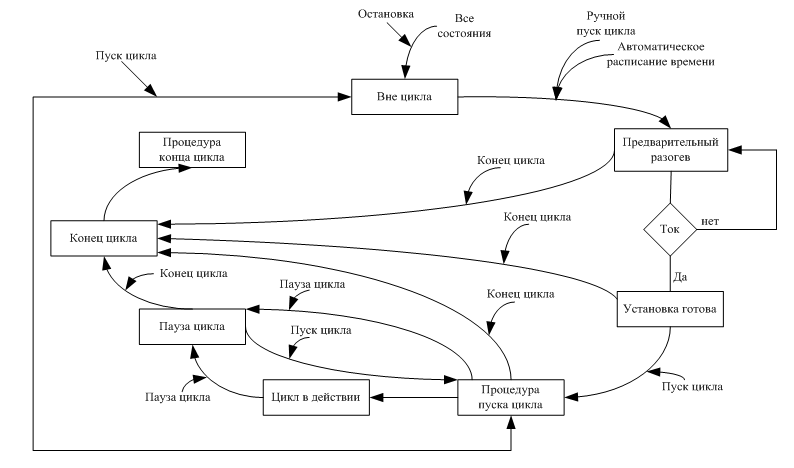
\includegraphics[scale=0.8]{images/part7/chapter_enterprise/line_ex.png}
	\caption{Пример схемы технологического цикла производства (линия эмалирования)}
	\label{fig:line_ex}
\end{figure}


Для описания управления технологической линией эмалирования введено понятие "цикл" работы. Термин "цикл" подразумевает производственную фазу, в течение которой линия эмалирования производит готовые детали.
Технологическая линия эмалирования считается готовой к производственной фазе или пуску "цикла" только после завершения этапа "предварительного разогрева". Во время предварительного разогрева все "горячие" участки линии эмалирования доводятся до режимной температуры.

Объектом моделирования является технологическая схема организации производства для изготовления элементов электроаппаратуры специального назначения, которая имеет графовую структуру и поэтому может быть формализована в рамках разработанной модели.

%(153)
Исходная информация для построения ИМ СУ ВТПП включает в себя множество параметров, характеризующих ее состав и структуру:
\begin{textitemize}
    \item количество реализаций имитационной модели ( $N$ ) согласно процедуре Монте-Карло;
    \item множество $\{X_i\}$ запросов ресурсов ВТТП, требуемых для выполнения исполнительных элементов системы управления;
    \item параметры коммутации исполнительных элементов с элементами синхронизации, генераторами входных сигналов и финальным элементом функционирования;
    \item множество $\{REL\}$ надежностных характеристик оборудования, с помощью которого осуществляется управление функционированием ВТПП;
    \item множество $\{ \lambda_j \}$ значений компонентов важности откликов имитации;
    \item вектор $\{ \delta_h \}$ коэффициентов важности откликов имитации;
    \item вектор {DEVLIST} конфигурации состава оборудовании, используемого в исследуемом варианте организации системы управления ВТПП.
\end{textitemize}

Для заполнения этих параметров производится мониторинг выполнения функций СУ ВТПП. Результаты обработки заполненных данных аппроксимируются некоторыми распределениями.

При выполнении множества микротехнологических операций ( $\{MTCO_{ij}\}$ ) согласно технологической схеме организации производства для формализации технологического цикла можно использовать вероятностный сетевой график, заменяя компоненты технологической схемы на операции и события выполнения операций в ИМ ВСГР. 

Многие операции изготовления элементов электроаппаратуры специального назначения используют оборудование индивидуального и общего пользования, которое может отказывать (а в ряде случаев могут возникать аварии на оборудовании). На оборудовании имеются специальные элементы индикации его использования и определения текущего состояния автоматики, регулирующей выполнение $\{MTCO_{ij}\}$. Кроме того, для повышения надежности функционирования оборудования может использоваться одиночное и групповое резервирование устройств. В экстренных ситуациях допускается переход оборудования на профилактику или ликвидацию последствий аварий оборудования.

Для управления динамикой выполнения $MTCO_{ij}$ и своевременного переключения оборудования на профилактику можно использовать имитационную модель ВСГР путем простой замены в ней устройств оборудования на агрегаты-имитаторы функционирования устройств оборудования общего и индивидуального пользования, а сами операции на ИМ ВСГР представить в имитационной модели набором агрегатов-имитаторов событий и агрегатов-имитаторов технологических операций.



\subsection{Решатели задач ostis-системы адаптивного управления вероятностным технологическим процессом производства}

При осуществлении процессов управления технологическим циклом  производства часто возникает потребность комплексного учета многообразия факторов воздействия на технологический процесс случайных сбоев используемого оборудования, а также воздействий внешней среды, включая и человеческий фактор. В этой связи является актуальной реализация адаптивного  управления  процессом  производства (с обратными связями по управлению)  в  составе технических средств управления технологическим циклом и программного обеспечения адаптации процесса управления на случайные внешние возмущения в ходе его реализации.

Адаптивное управление технологическим циклом понимается как способность системы управления адекватно реагировать на внешние возмущения и штатные управляющие воздействия изменением соответствующих параметров управления в процессе функционирования системы.

Под оптимальными управлением понимается формализованная нейронной сетью структура адаптивного управления технологическим циклом, построенная в опорных узлах вероятностной сетевой графовой структуры (СГС) или модели полумарковской сети (ПМС) в рамках заданного критерия качества.

Формализация процесса управления технологическим циклом производства с  вероятностными характеристиками основана на использовании в структуре контура управления специальных сигналов и стандартных элементов, которые в дальнейшем участвуют в формировании регулирующих воздействий непосредственно на используемое оборудование либо выдачи рекомендаций по выполнению определенных действий операторами-людьми.

Данные регулирующие воздействия (исполнение данных рекомендаций) могут приводить к изменениям параметров функционирования системы. Воздействия формируются в моменты изменения состояния ТЦ.

Необходимость оперативного изменения параметров функционирования системы возникает вследствие наличия внешних факторов; человеческого фактора, существования возможности возникновения отказов оборудования и аварий.

Система управления ТП связана с оборудованием ТП посредством средств программно-аппаратного сопряжения и в процессе реализации ТП получает сигналы о его состоянии. Изменение состояния ТП приводит к изменению состояния системы управления.

Для построения контроллера системы управления могут быть использованы статистические данные функционирования ТЦ, собранные с применением соответствующих средств аппаратно-программного сопряжения, либо может быть осуществлено использование имитационного моделирования функционирования ТЦ на базе модели ТЦ, построенной в соответствии с изложенной онтологией для технологических процессов с вероятностной природой.



\subsubsection{Проблемы адаптивного управления производственной деятельностью при разработке интеллектуальных компьютерных систем нового поколения}

Современный анализ состояния разработок в области исследования управляемых производственных систем показывает, что проблема определения параметров функционирования подобных объектов исследования в режиме реального времени возникает прежде всего при необходимости производства сложных технических изделий, требующих точности их изготовления и высокой производительности труда.

При этом в рамках решения многокритериальной задачи оптимизации управления предъявляются строгие требования к качеству и алгоритму выполнения производственного процесса, минимизации влияния человеческого фактора на качество реализации технологического цикла производства, исключению возникновения аварийных ситуаций техногенного характера. Подобная ситуация характерна для роботизированных производственных систем, работающих под управлением программно-аппаратного контроллера, который администрирует работу системы управления технологическим циклом в соответствии с заложенными программами.

Вместе с тем возникающие нештатные ситуации ввиду наличия сбоев оборудования, случайных внешних управляющих воздействий, включая и наличие человеческого фактора, приводят к отклонению параметров функционирования производственной системы от заданных, в связи с чем возникает необходимость корректировки параметров управления в режиме реального времени на основе моделей нейрорегуляторов, работающих в составе средств программного-аппаратного сопряжения с технологическим циклом производства.

Существующие специальные модели искусственного интеллекта, такие как нейронные сети, обладают уникальными свойствами, могут применяться в качестве универсальных аппроксиматоров, имеющих способность к обобщению. Эти особенности делают целесообразным применение моделей такого типа при решении сложных задач адаптивного управления.

Современное направление конвергенции работ в области создания интеллектуальных систем [golenkov mono] требует разработки соответствующего программного обеспечения с элементами когнитивных способностей на основе семантически совместимых технологий искусственного интеллекта. Данное направление включает в себя также создание компьютерных систем, обеспечивающих интеллектуализацию процессов принятия аналитических управленческих решений, что напрямую связано с адаптацией процессов управления сложными динамическими системами (техническими объектами) в режиме реального времени, созданием семантически совместимых баз знаний в области анализа функционирования динамических систем и оптимизации функционирования сложных технических систем на их основе посредством создания открытого программного кода интеллектуальных компьютерных систем поддержки принятия решений.



\subsubsection{Создание математической модели производственной системы в рамках концепции Industry 4.0}

Концепция Industry 4.0 была сформулирована в Германии в 2011 году. Она подразумевает создание и внедрение в производство т.н. киберфизических систем (КФС) и использование интернета вещей и услуг в производственных процессах (см. \scncite{Taberko2018}). При этом под КФС понимается совокупность интеллектуальных, легко интегрируемых физических компонентов со встроенными в них вычислительными ресурсами, тесно взаимодействующих между собой и отслеживающих изменения в состоянии внешнего мира.

Основные принципы концепции Industry 4.0:

\begin{textitemize}
\item \textbf{Взаимодействие}. Возможность взаимодействия устройств, датчиков, людей посредством Интернета вещей (IoT), Интернета людей (IoP), Интернета услуг (IoS).
\item \textbf{Виртуализация}. Означает способность киберфизической системы контролировать физические процессы. Данные сенсоров проецируются на модель предприятия, включающих состояние всех киберфизических систем. В случае возникновения нештатной ситуации должна быть возможность уведомить оператора, предоставив ему информацию по ее устранению и обеспечению безопасности, тем самым осуществляя поддержку принятия решений персоналом.
\item \textbf{Децентрализация}. Растущая потребность в штучных партиях заказных продуктов увеличивает сложность централизованного управления производством. КФС могут иметь встроенные вычислительные модули, позволяющие им принимать решения самостоятельно и переадресовывать задачу управляющей системе только в случае необходимости. Несмотря на это, необходимо обеспечить контроль качества конечного продукта и прослеживаемость, что требует централизованного управления. К примеру, необходимые шаги производственного процесса могут быть закодированы в RFID-метках, что освобождает от необходимости централизованного управления данным аспектом производства малых партий продукта.
\item \textbf{Анализ и реагирование в реальном времени}. С целью управления производством необходимо, чтобы данные с сенсоров постоянно собирались и анализировались в режиме реального времени. В случае отказа одной производственной установки, можно "перепоручить" её задачу другой.
\item \textbf{Ориентированность на услуги}. Услуги компаний, КФС и людей доступны в Интернете услуг и могут быть использованы другими участниками. Услуги могут предоставляться как внутри предприятия, так и другим предприятиям. КФС предоставляют свои услуги в виде веб-служб. Это позволит реализовать производство продукта путем комбинирования производственных операций в соответствии со спецификацией клиента, закодированной, например на RFID-метке.
\item \textbf{Модульность}. Система должна быть гибкой, т.е. легко адаптируемой к меняющимся требованиям (например, сезонным изменения в потреблении, изменению характеристик продукта или производства). Адаптация должна осуществляться заменой или расширением отдельных компонентов системы. Обеспечение совместимости компонентов требует наличия стандартизированных механизмов взаимодействия, позволяющих автоматически идентифицировать компоненты и включать их в интернет услуг.
Полная совокупность производственной деятельности предприятия может быть описана в качестве набора технологических процессов производства с вероятностными характеристиками в соответствие с описанной онтологией данной предметной области.
\end{textitemize}

Внедрение концепции Industry 4.0 на промышленных предприятиях сопровождается построением единой онтологической модели производства, которая является ядром комплексного информационного обслуживания предприятия (см. \scncite{Savushkin2020a}). Потребность в комплексной автоматизации сложных процессов, требующих согласованной работы множества служб и технических средств, создает потребность в разработке систем, осуществляющих интеграцию вычислительных ресурсов и физико-технических процессов.

Для того чтобы обеспечить широкое применение технологий искусственного интеллекта в автоматизации предприятия, все корпоративные знания предприятия должны быть записаны на формальном языке представления знаний. Источниками таких знаний могут служить существующие описания работы предприятий в рамках принятых международных стандартов. В результате реализации онтологической модели предприятия возникает возможность интеграции и применения систем и подходов различной природы для автоматизации различных аспектов производственной деятельности.

Онтологическая модель производственной системы при этом включает в себя модели производственных процессов данного предприятия, которые можно представить в описанной в данной главе формализации. 


\subsubsection{Разработка моделей нейрорегуляторов для решения задач адаптивного управления в условиях Экосистемы OSTIS}

В рамках решения задачи адаптивного управления в изложенной формализации может быть предложено несколько подходов:

\begin{textitemize}
    \item Прямое управление с эталонной моделью (последовательная схема управления), при котором путем обучения нейронной сети на базе существующих "оптимальных"{} сигналов системы управления (см. \scncite{Omidvar1997}), приводящих к формированию желаемых траекторий в фазовом пространстве системы, строится нейросетевой контроллер системы управления (\scncite{Smorodin2019}). Данная схема  нейроуправления является наиболее простой, но имеет недостатки в виде необходимости наличия репрезентативной выборки статистики работы существующего физического контроллера.
    
    \item Прямое инверсное управление (см. \scncite{White1992}), при котором нейроконтроллер обучается воспроизводить зависимость между управляющим сигналом в текущий момент времени и наблюдениями за объектом управления в следующий момент времени в процессе моделирования функционирования контура управления, такой подход показан в работах \scncite{Ivaniuk2013} \scncite{Ivaniuk2014}. 
    
    
    \item Могут быть предложены схемы построения нейроконтроллеров на основе обучения с подкреплениям, в частности:
    \begin{textitemize}
        \item  Управление с помощью нейросетевого контроллера, сформированного через процедуру обучения с подкреплением на задаче поиска в некотором ("геометрическом") смысле оптимальной траектории в фазовом пространстве системы управления в явном виде (см. \scncite{Hagan1999} \scncite{White1992} \scncite{Smorodin2019a}).

        \item  Управление с помощью нейросетевого контроллера, сформированного через процедуру обучения с подкреплением на задаче неявного поиска оптимальной траектории путем максимизации определенной оценки качества управления $R$ (см. \scncite{Smorodin2020}, \scncite{Smorodin2022}).    
    
    \end{textitemize}

\end{textitemize}

Поскольку задача подбора структуры нейронной сети в каждом из случаев является сложной и трудноформализуемой, перспективным направлением является использование эволюционных методов для ее автоматизации (см. \scncite{Stanley2002}). 

\subsubsection{Формализация управления технологическим циклом производства на основе применения ostis-систем}

В соответствие с изложенной онтологией под технологическим циклом производства подразумевается последовательность действий и операций, в результате которых осуществляется производство готовой продукции.

Функциональное взаимодействие компонентов комплекса управления и работающего в режиме реального времени технологического цикла производства осуществляется на основе непрерывного мониторинга состояния оборудования и параметров управления с помощью регистров-индикаторов и технических средств сопряжения.


С целью обеспечить возможность интеграции различных моделей (включая нейросетевые) с другими интеллектуальными системами предлагается формализация системы принятия решений на базе Технологии OSTIS.





\subsubsection{Принципы оптимизации процессов управления технологическим циклом с использованием нейросетевого моделирования}

При управлении с эталонной моделью ставится задача построения такого нейросетевого контроллера таким образом, чтобы происходило приемлемое обобщение собранных массивов данных об управлении технологическим циклом. С точки зрения теории машинного обучения в этом случае будет решаться задача обучения с учителем, при которой собранные данные будут использованы в качестве пар эталонных векторов входов и выходов контроллера (управляющих сигналов контроллера). С точки зрения теории динамических систем фазовое пространство состояний системы управления ТП – среда, в которой на основании наблюдаемого состояния необходимо принимать решения о выборе текущего управления. И поэтому процесс обучения нейронной сети можно рассматривать как процесс запоминания корректных траекторий в фазовом пространстве, соответствующим оптимальным управлениям. 



Процесс обучения при инверсной схеме является схожим с точки зрения теории машинного обучения, с той разницей, что источником формирования оптимизируемой функции потерь являются желаемые сигналы наблюдений за объектом управления.

\begin{figure}[H]
	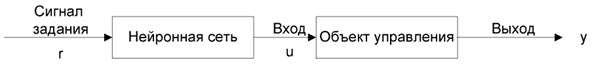
\includegraphics[scale=0.8]{images/part7/chapter_enterprise/nncontrol_direct.png}
	\caption{Схема прямого управления технологической системой}
	\label{fig:nncontrol_direct}
\end{figure}

\begin{figure}[H]
	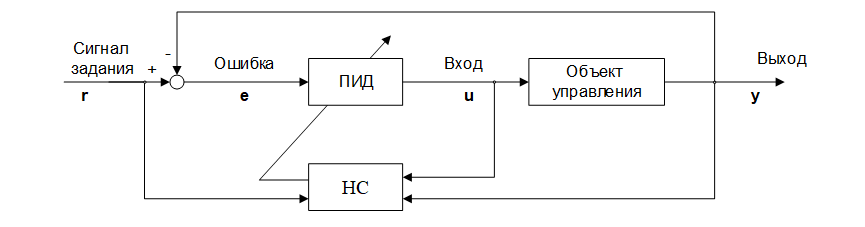
\includegraphics[scale=0.8]{images/part7/chapter_enterprise/nncontrol_inverse.png}
	\caption{Пример реализации схемы с инверсным управлением}
	\label{fig:nncontrol_inverse}
\end{figure}

Возможен подход при котором применяются методы обучения с подкреплением для построения эффективного контроллера системы управления. Методы обучения с подкреплением подразумевают исследовательское поведение агента в процессе построения контроллера, что может иметь позитивный эффект при решении задач со сложной структурой принятия управляющих решений.

Пусть задан некоторый функционал оценки качества управления $R$ (качества выбора политики управления (выбора агентом (системой управления) действий) $\pi$), рассчитываемый на промежутке времени реализации вероятностного сетевого графика ТП $[0,t]$. (Данный функционал может "награждать", например, за снижение издержек производства, "штрафовать" за простой оборудования, возникновения отказов оборудования либо аварий.)

Принятие решений в этой среде может осуществляться нейронной сетью (агент под управлением нейросетевого контроллера).

Совершение агентом некоторых действий в фазовом пространстве системы управления приводит к построению некоторой траектории (в данном контексте построение управления рассматривается как построение траектории в фазовом пространстве системы управления технологического процесса производства).


Задача поиска оптимальной траектории в фазовом пространстве системы, таким образом, сводится к максимизации $R$ (как в текущий момент, так и в будущем – т.е. к контроллеру системы управления ТЦ предъявляется требование формирование политики выбора действий $\pi$, максимизируещей оценку качества управления $R$).

Можно выделить две группы алгоритмов обучения с подкреплением, используемые для решения сложных задач управления:

\begin{enumerate}
    \item ``value-based'' – обучение контроллера оценке функции будущего вознаграждения;
    \item ``policy-based'' – обучение контроллера распределению действий, приводящих к выбору оптимальной политики.
\end{enumerate}


Применение методов обучения с подкреплением подразумевает создание среды, в которой агент совершает действия. Агент совершает действия на основания текущего набора наблюдений за средой, а по результату совершения действий и последовавшего за ним возможного изменения состояния среды, получает численную награду.


Средой, в которой действует агент, в контексте решения задач управления технологическим циклом является система управления технологическим циклом производства, которая делает доступным для агента наблюдение за сигналами регистров о состоянии оборудования и параметров управления. На основании решений агента система принятия решений формирует запросы на изменения параметров управления.


В контексте применения подходов к построению контроллера системы управления, основанных на обучении с подкреплением могут быть предложены следующие методы к организации среды, в которой действует и обучается агент:

\begin{enumerate}
    \item использование наблюдений за функционированием физического технологического процесса, при котором имплементированы схемы сравнения действий физической системы управления с действиями, предложенными агентом, с оценкой их соответствия текущей ситуации и допустимостью
    \item использование имитационного моделирования технологического процесса производства в качестве базы для построения среды для обучения с подкреплением
\end{enumerate}



\subsubsection{Построение фазовой плоскости (фазового пространства) состояний системы адаптации управления технологическим циклом производства}

Фазовое пространство состояний системы управления ТП – среда, в которой на основании наблюдаемого состояния необходимо принимать решения о выборе текущего управления. Анализ фазового пространства состояний позволяет рассматривать задачу управления в геометрическом контексте. 


\subsubsection{Алгоритмы адаптации управления технологическим циклом при использовании нейросетевого моделирования}

Процесс обучения нейронной сети заключается в поиске таких значений настраиваемых параметров сети (весовых коэффициентов связей между нейронами и уровней активации нейронов), чтобы она осуществляла правильное отображение. Обучение часто можно рассматривать как нелинейную оптимизационную задачу минимизации некоторой функции потерь относительно настраиваемых параметров сети. Форма этой функции определяется постановкой задачи, решаемой с применением нейронной сети.

При подходе, основанном на управлении с эталонной моделью, нейроконтроллер обучается с учителем. При этом используется функция потерь, оценивающая отклонение выходных сигналов сети от эталонных, и производится оптимизация данной функции (обычно градиентными методами).


Q-обучение  является примером ``value-based'' алгоритма обучения с подкреплением, который может быть применен для поиска настраиваемых параметров модели при решении задач управления технологическим циклом.


Идея Q-обучения состоит в том, что агент в процессе обучения строит верную функцию Q оценки вознаграждения за следующее состояние, к которому может привести выбор некоторого управления (см. \scncite{Watkins1992}).


Функция вознаграждения при этом основана на оценке качества управления контроллера. Определение функции вознаграждения играет важную роль, определяя поведение агента, формируемое при обучении. Выбор функции вознаграждения позволяет выбрать для оптимизации те критерии поведения агента, которые пользователь системы считает важными.


В качестве аппроксиматора функции вознаграждения может быть использована нейронная сеть. В этом случае задачей обучения является поиск таких значений настраиваемых параметров нейросети, при которых приближенная функция $Q$ будет достаточно близкой к оптимальной функции $Q*$ при данной политике выбора действий $\pi$ (см. \scncite{Mnih2015}):


$Q^{*}(s,a)=\mathbb{E}(r+\gamma \max_{a'}Q^{*}(s',a')|s,a) $


для которой выполняется уравнение Беллмана:

$Q(s,a)\approx Q^{*}(s,a)=\max_{\pi}\mathbb{E}\left [ R_t|s_t=s,a_t=a \right ]$

При решении сложных практических задач агенту часто бывает недоступна полная информация о состоянии среды. В этой ситуации агент, который пользуется аппроксиматором $Q$, зависящим только от текущего наблюдаемого состояния среды может быть неэффективным при достаточно сложной структуре среды или наличии в ней распределенных во времени процессов, как связанных с действиями агента, так и независимыми от них. В описанной ситуации возможно использование в качестве аппроксиматора рекуррентной нейросети, обладающей внутренним состоянием (см. \scncite{Bakker2001}). LSTM-блоки (предложенные в работе \scncite{Hochreiter1997}), при использовании в рекуррентной сети позволяют ей аппроксимировать сложные зависимости, растянутые на длительные периоды времени.


В policy-based методах вместо аппроксимации числовой функции, оценивающей возможные награды получаемые в окружении агентом за совершенные действия, происходит построение напрямую функции политики выбора действий, связывающей состояния с действиями агента. Имеет место параметризации политики выбора действий настраиваемыми параметрами модели, под управлением которой функционирует агент.

Численная функция (функция награды) при этом может быть использована для оптимизации политики относительно настраиваемых параметров, но не используется для выбора действий.

Стохастическая политика выбора действий возвращает распределение вероятностей возможных действий. Такие политики используются в частично наблюдаемых окружениях при наличии неопределенности.


Было показано, что для определенных классов задач методы, основанные на политиках сходятся быстрее чем value-based (Q-обучение), предпочтительны в пространствах выбора действий высокой размерности (см. \scncite{Sutton1998}). Гарантируется сходимость по крайней мере к локальному максимуму качества.


Политика $\pi$ параметризована настраиваемыми параметрами $\theta$.

$\pi_{\theta} (a|s)= P[a|s]$

Эта политика возвращает распределение действий a при наблюдаемом состоянии среды $s$.

С целью поиска настраиваемых параметров необходимо решить оптимизационную задачу максимизации функции оценки качества $J( \theta )$ .

$J( \theta )=E_{ \pi  \theta } ( \sum  \gamma r)$

Правила обновления настраиваемых параметров на шаге t:

$\theta _{(t+1)} := \theta _{t}+ \alpha  \bigtriangledown J( \theta _t)$


Согласно Policy Gradient Theorem[5]

$\bigtriangledown E_{ \pi  \theta } (r( \tau ) )=E_{ \pi  \theta } (r( \tau ) \bigtriangledown log \pi _{ \theta  ( \tau )})$


что может быть преобразовано как

$\bigtriangledown E_{ \pi  \theta } (r( \tau ) )=E_{ \pi  \theta } (r( \tau )( \sum_{t=1}^{T}  \bigtriangledown log  \pi _{ \theta } (a_t |s_t)))$


Алгоритм REINFORCE, предназначенный для изучения агентом политики выбора действий, приводящей к максимизации кумулятивных будущих наград, может быть сформулирован следующим образом\cite{Sutton1998}:

\begin{enumerate}
    \item Инициализировать параметры политики $\theta$
    \item Сгенерировать эпизод взаимодействия агента со средой с $\{S_i \}$, $\{A_i \}$, $\{R_i \}$   – последовательностями наблюдаемых агентом состояний среды, выборов действий, полученных наград длинной T.
    \item Для каждого шага t вычислить discounted reward $G_t :=  \sum_{k=t+1}^{T}   \gamma ^{k-t-1} R_k  $
    \item Обновить параметры по правилу $\theta :=  \theta + \alpha  \gamma ^t G \bigtriangledown_ \theta  ln \pi (A_t |S_t, \theta )$
    \item Повторить шаги 2-4 до сходимости.


\end{enumerate}


\subsubsection{Решатели задач ostis-системы адаптивного управления технологическим циклом производства}

В рамках Технологии OSTIS решатели задач строятся на базе мультиагентного подхода. В соответствии с этим подходом решатель задачи строится как набор агентов, называемых sc-agents. Все такие агенты разделяют память и могут обмениваться данными через специальные семантические структуры (sc-texts). Важно отметить, что некоторые агенты могут быть неатомарными, т.е. представленными в виде двух или более sc-агентов.

Полный решатель для задачи управления может быть представлен как разложение абстрактного неатомарного sc-агента.


\begin{SCn}
\scnheader{abstract non-atomic sc-agent of cycle recommendation system}
\begin{scnrelfromset}{decomposition of abstract sc-agent}
    \scnitem{abstract sc-agent of interaction with the observation system}
    \scnitem{abstract sc-agent of forming recommendations}
    \scnitem{abstract sc-agent of forming requests}
\end{scnrelfromset}
\end{SCn}

\begin{enumerate}
    \item abstract sc-agent of interaction with the observation system – предназначен для извлечения наблюдений из средств аппаратно-программного сопряжения в технологическом цикле, инициирует работу агента, ответственного за формирование рекомендаций.
    \item abstract sc-agent of forming recommendations – на основании полученных наблюдений инициирует работу контроллера для получения рекомендаций по осуществлению управляющих воздействий.
    \item abstract sc-agent of forming requests – на основании данных полученных от агента формирования рекомендаций, формирует запросы на  изменения переменных управления ВТП посредством соответствующих программно-аппаратных средств сопряжения.

\end{enumerate}

Построение контроллера, используемого в 2) может быть осуществлено на базе нейронных сетей.



\subsubsection{Система адаптации управления}

При разработке  системы адаптации управления в рамках построения решателя задач ostis-системы предложенной структуры, необходимо реализовать агент для формирования рекомендаций на основании полученных наблюдений. В основе данного агента лежит контроллер, сформированный в соответствие с одним из алгоритмов, описанных выше.



\subsubsection{Примеры реализации систем адаптации управления}

В качестве примера можно рассмотреть задачу поиска оптимальной стратегии обслуживания оборудования технологического цикла производства (см. \scncite{Smorodin2022}).

Решатель такой задачи может быть представлен как разложение абстрактного неатомарного sc-агента.

\begin{SCn}
\scnheader{abstract non-atomic sc-agent of cycle maintenance recommendation system}
\begin{scnrelfromset}{decomposition of abstract sc-agent}
    \scnitem{abstract sc-agent of interaction with the observation system}
    \scnitem{abstract sc-agent of forming recommendations}
    \scnitem{abstract sc-agent of forming maintenance requests}
\end{scnrelfromset}
\end{SCn}

\begin{enumerate}
    \item abstract sc-agent of interaction with the observation system – предназначен для извлечения наблюдений из средств аппаратно-программного сопряжения в технологическом цикле, инициирует работу агента, ответственного за формирование рекомендаций.
    \item abstract sc-agent of forming recommendations – на основании полученных наблюдений инициирует работу нейроконтроллера для получения рекомендаций по совершению операций обслуживания.
    \item abstract sc-agent of forming maintenance requests – на основании данных полученных от агента формирования рекомендаций, формирует запросы на обслуживание для соответствующих программно-аппаратных средств сопряжения.

\end{enumerate}

Для построения нейроконтроллера будет использовано обучение с подкреплением. В качестве среды для обучения с подкреплением будет использоваться имитационная модель технологического цикла производства.

Для реализации имитационной модели в описанной формализации используются:


%!!! ЗАМЕНИТЬ ОБОЗНАЧЕНИЯ НА ТАКИЕ ЖЕ КАК В ПЕРВОЙ ПОЛОВИНЕ | +

\begin{textitemize}
    \item распределения длительности безотказной работы для оборудования $i$-го типа $\Phi_{1r}^i(\tau_{NOr})$  в режиме $r(M_i)$;
    \item распределения длительности восстановления (ремонта) оборудования i-го типа после отказа $\Phi_{2r}^i(\tau_{ROr})$ ;
    \item распределения длительности ликвидации аварии на оборудовании i-го типа $\Phi_{3r}^i(\tau_{em1})$ ;
    \item вероятности возникновения аварии при отказе $i$-го узла $\Phi_{4r}^i(C_{em1})$.
\end{textitemize}


Имитационная модель функционирует в течение заданного интервала времени, перезапуская производственный цикл и, возможно, осуществляя перед этим запуском профилактические действия. Для принятия решения о проведении и содержании профилактических действий используется система управления технологическим циклом.


Система управления технологическим циклом производства делает доступным для агента наблюдение за временем безотказной работы всех узлов $M_i$.


Формирование функции вознаграждения включает такие компоненты как время непрерывной работы цикла($R_{nop}$), суммарный объём затрат на обслуживание и ликвидацию отказов и аварий оборудования($R_{cost}$), суммарное число отказов оборудования ($R_{f}$), в том числе, приведшее к аварии ($R_{fe}$), суммарное число профилактик за цикл ($R_{rep}$). В процессе обучения модели значение функции вознаграждения формируется следующим образом во время единичного прохождения процедуры ``профилактика-цикл''. Каждый из компонентов награды входит в уравнение с заданным весовым коэффициентом $\alpha_i$, характеризующим его значимость.


$R=\alpha_1 R_{nop}+\alpha_2 R_{cost}+\alpha_3 R_{f}+\alpha_4 R_{fe}+\alpha_5 R_{rep}$

Для управления агентом использованы нейросети на базе МСП с блоком LSTM. В случае с policy gradient используется sigmoid, выход сети представляет собой распределение вероятностей действий.
Структура сети:

\begin{enumerate}
    \item Dense x64 ReLU
    \item Dense x64 ReLU
    \item LSTM x32 ReLU
    \item Dense x6 softmax

\end{enumerate}

В качестве другого примера решения задачи адаптивного управления, с использованием нейросетевых подходов, можно рассмотреть задачу стабилизации температуры в процессе функционирования пластинчатой пастеризационно-охладительной установки (ПОУ) (см. \scncite{Ivaniuk2014}). ПОУ предназначена  для  тепловой  обработки  и  охлаждения  молочных продуктов  в  непрерывном  тонкослойном  закрытом  потоке. Для  автоматизации  регулирования  температурного  режима  в  состав  ПОУ входит  система  управления  на  базе  промышленного  контроллера. От  применяемых  алгоритмов  управления  напрямую  зависит  качество получаемой продукции.

Основными  причинами,  вызывающими  колебания  температуры $t_{mn}$ нагревания молока являются непостоянство расхода $G_m$ продукта, непостоянство температуры $t_0$ исходного молока, изменение расхода $G_p$  пара,  обусловленное  колебания  его  давления $P_{pr}$, изменение коэффициента теплопередачи K вследствие отложения белка молока на теплопередающих поверхностях. Для стабилизации температуры $t_{mn}$ нагревания молока в качестве управляющего воздействия в основном применяют расход пара $G_p$. Его регулируют посредством управляемого клапана.

Общая структура самонастраивающегося  нейро-ПИД  регулятора  показана  на  рисунке ниже, где выходами нейронной сети – являются пропорциональный ($K_P$), интегральный ($K_I$) и дифференциальный ($K_D$) коэффициенты.

\begin{figure}[H]
	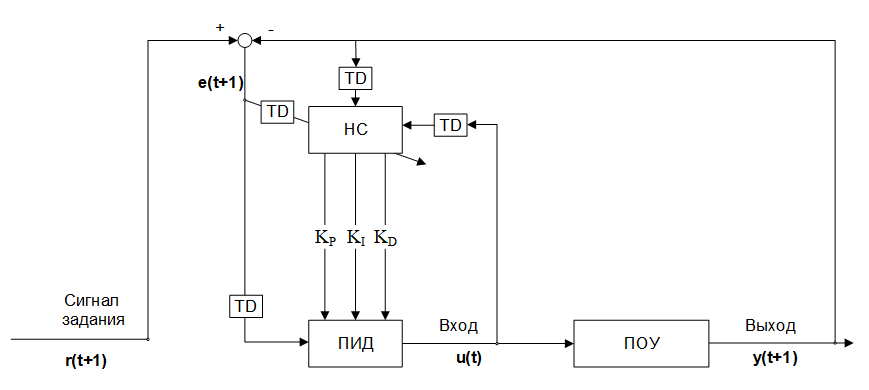
\includegraphics[scale=0.8]{images/part7/chapter_enterprise/neuropid.png}
	\caption{Общая структура  нейро-ПИД  регулятора}
	\label{fig:neuropid}
\end{figure}


ПИД-регулятор в дискретном времени описывается следующим выражением

$u_n = u_{n-1} + K_p (e_n - e_{n-1}) + K_I e_n + K_D (e_n - 2e_{n-2}+ e_{n-2} )$

где $K_P$, $K_I$ и $K_D$ – пропорциональный, интегральный и дифференциальный коэффициенты соответственно, $u_n$ определяет вход объекта управления в момент $t = nT_0$ и $e_n$ – ошибка между желаемым значением выхода $r_n$ и реальным, то есть 

$e_n = r_n - y_n $

,$T_0$ определяет единичный интервал времени. 

Для настройки $K_P$, $K_I$ и $K_D$ во время работы мы будем использовать  трехслойный  персептрон.  Каждый  слой  состоит  из $N_1$, $N_2$ и $N_3$ нейронов соответственно. Количество нейронов выбирается  исходя  из  экспертного  опыта  и  сложности  объекта  управления, $N_3$ равняется трем – количество коэффициентов ПИД. Для использования алгоритма обратного распространения ошибки мы должны выбрать функцию $E$, значение которой должно быть минимизировано. В качестве такой функции будет выступать ошибка управления neв момент времени $nT_0$.

$E_n = 1/2 e^2_n$ 

Для накопления ошибок сохраняем полученные ранее данные – $E_{n-p}, ..., E_{n-2},E_{n-1},E_n$,  где $p$  определяет  количество  сохраненных ранее образов, используемых для обучения сети.



\section{Построение умных предприятий рецептурного производства с помощью ostis-систем}


\subsection{Проблемы проектирования умных предприятий}


\subsubsection{Проблемы разработки систем комплексной автоматизации}

Существующие средства автоматизации деятельности предприятия имеют высокую стоимость, трудны в освоении и адаптации к конкретному производству. Как правило, такие средства, с одной стороны, жёстко ориентированы на решение некоторого ограниченного класса задач, с другой стороны, разработчики стремятся сделать такого рода средства как можно более универсальными, наращивая их частными решениями, что приводит к сложности и громоздкости таких систем. Вследствие подобного подхода к наращиванию функционала существующие средства автоматизации деятельности предприятия имеют низкий уровень гибкости (возможности внесения изменений), что приводит к существенным накладным расходам при адаптации таких средств к новым требованиям. Как правило, внесение изменений в указанные средства требует вмешательства разработчиков (часто сторонних с точки зрения предприятия), что влечёт значительные временные и финансовые затраты. Как следствие указанных проблем, далеко не всякое предприятие может обеспечить высокий уровень автоматизации своей деятельности, даже в случае наличия на рынке подходящих решений (см. \scncite{Savushkin2017}, \scncite{Savushkin2017a}).
Отсутствие общих унифицированных моделей и средств построения систем автоматизации деятельности предприятия приводит к большому количеству дублирований аналогичных решений как в рамках различных предприятий, так и в рамках разных подразделений одного предприятия. При этом часто возникает ситуация, когда некоторые частные системы, решающие различные задачи в рамках одного предприятия, оказываются несовместимыми между собой, что приводит к дополнительным расходам на реализацию механизмов согласования, например, преобразование форматов данных. Отсутствие такого рода моделей препятствует дальнейшему повышению уровня автоматизации предприятия, в частности, в области автоматизации принятия решений в нештатных ситуациях, прогнозирования дальнейшего развития событий.

\subsubsection{Требования, предъявляемые к стандартизации предприятий}

Средства автоматизации предприятия должны оперативно и с минимальными затратами времени сотрудников адаптироваться к любым изменениям самого производства – к расширению или сокращению объёмов производства, изменениям номенклатуры производства, изменению используемого оборудования, изменению общей структуры производства, изменению взаимодействия с поставщиками и потребителями, к изменению нормативно-правовых актов (включая стандарты), к различного рода непредвиденным обстоятельствам.
Адаптация средств автоматизации предприятия ко всем видам изменений самого предприятия и всем аспектам его взаимодействия с внешней средой требует внесения изменений в модель предприятия, полностью отражающую текущее состояние его деятельности.
Средства автоматизации предприятия должны быть гибкими не только для оперативной адаптации к реконфигурации производства, но и для оперативного внесения изменений в сами средства автоматизации в направлении их постоянного совершенствования. Здесь существенным является не только снижение трудоёмкости повышения уровня автоматизации, но и поддержка высоких темпов повышения уровня автоматизации, а также чётко продуманный переходный процесс от одного уровня автоматизации к следующему, в ходе которого одновременно используется и устаревший вариант, и новый.
Эксплуатация системы автоматизации предприятия текущего уровня и перманентный процесс повышения этого уровня требуют согласованного и квалифицированного взаимодействия сотрудников предприятия. Основой такого взаимодействия является хорошо структурированная, достаточно полная и оперативно актуализируемая модель предприятия, отражающая все аспекты текущего состояния структуры и деятельности предприятия, а также планы его развития. Такого рода комплексная модель называется знаниями предприятия, которыми надо управлять (добывать, хранить, модернизировать, распространять и т.д.).
Повышение уровня автоматизации предприятия предполагает существенное расширение числа автоматически или автоматизированно решаемых задач, а это, в свою очередь, приводит к автоматизации решения интеллектуальных задач, т.е. к использованию технологий искусственного интеллекта. К числу интеллектуальных задач, решаемых на предприятии, можно отнести:
\begin{enumerate}
    \item анализ производственных ситуаций (в том числе нештатных);
    \item принятие решений на различных уровнях;
    \item планирование поведения в сложных обстоятельствах;
    \item генерация, актуализация документации;
    \item обучение новых и повышение квалификации действующих сотрудников;
    \item и т.д.
\end{enumerate}
Для того, чтобы обеспечить широкое применение технологий искусственного интеллекта в автоматизации предприятия, все корпоративные знания предприятия должны быть записаны на формальном языке представления знаний. При этом указанный язык должен быть удобен не только для использования в интеллектуальных компьютерных системах, но и для использования всеми сотрудниками предприятия.

\subsubsection{Проблемы стандартизации в области производственной деятельности}

Анализ работ в данной области позволил сформулировать наиболее важные и общие проблемы, связанные с разработкой и применением современных стандартов в различных областях:
\begin{textitemize}
    \item Прежде всего сложность ведения самих стандартов из-за дублирования информации, особенно сложность изменения терминологии.
    \item Дублирующаяся информация в документации, описывающей стандарт.
    \item Проблемы интернационализации стандартов -- перевод стандарта на несколько языков фактически требует поддержки и координации независимых версий стандарта на разных языках.
    \item В результате несоответствия форматов разных стандартов. В результате автоматизация процесса разработки и применения стандартов усложняется.
    \item Неудобство использования стандарта, особенно сложность поиска нужной информации. Как следствие, сложность изучения стандартов.
    \item Сложность автоматизации проверки соответствия объекта или процесса требованиям определенного стандарта.
    \item etc.
\end{textitemize}

Эти проблемы в основном связаны с представлением стандартов. Наиболее перспективным подходом к решению этих задач является преобразование каждого конкретного стандарта в базу знаний, в основе которой лежит набор соответствующих этому стандарту онтологий. Такой подход позволяет значительно автоматизировать процессы разработки стандарта и его применения.

В качестве примера рассмотрим стандарт \textbf{\textit{ISA-88}} \cite{ISA88} (базовый стандарт для рецептурного производства). Хотя этот стандарт широко используется американскими и европейскими компаниями и активно внедряется на территории Республики Беларусь, он имеет ряд недостатков, перечисленных ниже. Опыт автора со стандартами ISA-88 и ISA-95 выявил следующие проблемы, связанные с версиями стандарта (см. \scncite{Savushkin2022}):
\begin{enumerate}
    \item Американская версия стандарта -- \textit{ANSI/ISA-88.00.01-2010} -- была обновлена и находится в третьем издании 2010 года;
    \item \textit{ISA-88.00.02-2001} – содержит структуры данных и рекомендации для языков;
    \item \textit{ANSI/ISA-TR88.00.02-2015} -- описывает пример реализации ANSI/ISA-88.00.01;
    \item \textit{ISA-88.00.03-2003} -- действие, описывающее использование общих рецептов сайта внутри и между компаниями;
    \item \textit{ISA-TR88.0.03-1996} -- показывает возможные форматы представления процедур рецепта;
    \item \textit{ANSI/ISA-88.00.04-2006} -- структура записей серийного производства;
    \item \textit{ISA-TR88.95.01-2008} -- объясняет совместное использование ISA-88 и ISA-95;
    \item В то же время европейская версия, утвержденная в 1997 году -- \textit{IEC 61512-1} -- основана на более старой версии \textit{ISA-88.01-1995};
    \item Русская версия стандарта -- \textit{ГОСТ Р МЭК 61512-1-2016} -- идентична \textit{МЭК 61512-1}, то есть также устарела. Также вызывает ряд вопросов, связанных с не очень удачным переводом оригинальных английских терминов на русский язык.
\end{enumerate}

Другим стандартом, часто используемым в контексте Индустрии 4.0, является \textit{\textbf{ISA-95}} \cite{ISA95}. \textit{\textbf{ISA-95}} -- это отраслевой стандарт для описания систем управления высокого уровня. Его основная цель — упростить разработку таких систем, абстрагироваться от аппаратной реализации и предоставить единый интерфейс для взаимодействия со слоями ERP и MES. Состоит из следующих частей (см. \scncite{Savushkin2022}):
\begin{enumerate}
    \item \textit {ANSI/ISA-95.00.01-2000}, Часть 1: ``Модели и терминология'' — состоит из стандартной терминологии и объектных моделей, которые можно использовать для определения того, какая информация подлежит обмену;
    \item \textit {ANSI/ISA-95.00.02-2001}, Часть 2: ``Атрибуты объектной модели'' — он состоит из атрибутов для каждого объекта, определенного в части 1. Объекты и атрибуты могут использоваться для обмена информацией между различными системами, а также могут использоваться в качестве основы для реляционных баз данных;
    \item \textit {ANSI/ISA-95.00.03-2005}, Часть 3: ``Операционные модели управления производством'' — основное внимание уделяется функциям и действиям Уровня 3 (Производство/MES);
    \item \textit {ISA-95.00.04} Часть 4: ``Объектные модели и атрибуты для операций управления производством''. Комитет SP95 все еще разрабатывает эту часть ISA-95. Эта техническая спецификация определяет объектную модель, которая определяет обмен информацией между действиями MES (определено в Части 3 стандарта ISA-95). Модель и атрибуты Части 4 составляют основу для разработки и внедрения стандартов интерфейса, обеспечивая гибкий поток сотрудничества и обмена информацией между различными видами деятельности MES;
    \item \textit {ISA-95.00.05} Часть 5: ``Транзакции между бизнесом и производством (B2M транзакции)''. Часть 5 стандарта ISA-95 все еще находится в разработке. Эта техническая спецификация определяет операции между рабочими местами и структурами автоматизации производства, которые могут использоваться вместе с моделями элементов частей 1 и 2. Операции объединяют и упорядочивают описанные производственные элементы и действия. в рамках предыдущей части стандарта.Такие операции возникают в любом отношении внутри организации, однако внимание данной технической спецификации уделяется взаимодействию между организацией и системой управления.
    \item \textit {ISA-95.00.06} Часть 6: ``Транзакции между производственными операциями''.
    \item \textit {ISA-95.00.07} Часть 7: ``Модель сервисных сообщений''.
    \item \textit {ISA-95.00.08} Часть 8: ``Профили обмена информацией''
\end{enumerate}

Модели помогают определить границы между бизнес-системами и системами управления. Они помогают ответить на вопросы о том, какие функции могут выполнять какие задачи и какой информацией необходимо обмениваться между приложениями.

Первый этап построения модели цифрового двойника требует встраивания данных на более низких уровнях производства, таких как производственные процессы и оборудование (см. \scncite{Lutska2022}). Схема производства P\&ID служит источником этих данных. Поэтому стандарт ISA 5.1 \cite{ISA_5_1} должен работать со схемой P\&ID и широко используется в системах управления наряду со стандартом ISA 88 для полного описания нижних уровней производства. Этот стандарт полезен, когда требуется ссылка на оборудование в химической, нефтяной, энергетической, кондиционирующей, металлообрабатывающей и многих других отраслях промышленности. Стандарт позволяет любому человеку с достаточным уровнем знаний о предприятии читать блок-схемы, чтобы понять, как измерять и контролировать процесс, не вдаваясь в детали приборов или знаний эксперта по приборам. Он предназначен для предоставления достаточной информации, чтобы SA5.1 Целью настоящего стандарта было установить последовательный метод наименования приборов и контрольно-измерительных систем, используемых для измерения и контроля. Для этого представлена система обозначений, включающая символы и идентификационные коды. Последним выпуском подкомитета ISA5.1 является обновленный \textit {ISA-5.1-2022}, ``Символы приборов и идентификация''.

Обучение — это простой способ достичь этих стандартов. Международное общество автоматизации (\textit {ISA}) — некоммерческая профессиональная ассоциация и признанный лидер в области обучения автоматизации и управлению, занимающийся подготовкой рабочей силы к технологическим изменениям и отраслевым вызовам. Однако цена относительно высока, около 1000 долларов на человека в день. Для 2 человек это 10000\$ за обычный курс на 5 дней. Для одних стран это доступно, для других нет.

Принимаются во внимание различные установленные процедурные требования различных организаций, но это делается путем предоставления альтернативных методов символики, если это не противоречит целям стандарта. Существует множество вариантов добавления информации или упрощения символа при желании.

Эти и другие стандарты сейчас распространяются в виде документов, неудобных для автоматизированной обработки и, как отмечалось выше, сильно зависят от языка, на котором написан каждый документ.

\subsection{Подходы к проектированию и стандартизации умных предприятий рецептурного производства с помощью ostis-систем}


\subsubsection{Подходы к автоматизации предприятий}

В настоящее время существует ряд подходов, ориентированных на повышение уровня автоматизации и гибкости предприятий различного рода. Рассмотрим те из них, которые оказали влияние на развитие подхода, предлагаемого в данной работе (см. \scncite{Savushkin2017}, \scncite{Savushkin2017a}).
\begin{textitemize}
    \item Онтологические модели предприятий. Подход к проектированию различного рода систем на основе онтологических моделей широко используется в настоящее время, при этом в особую область исследований выделяют ``онтологии предприятия''. Суть предлагаемых подходов состоит в построении онтологий, описывающих деятельность того или иного предприятия или его подразделений. Недостатками данных моделей являются отсутствие унификации представления различных видов знаний предприятия, отсутствие единого подхода к выделению и формированию онтологий, отсутствие единого подхода к построению иерархии онтологий, что ограничивает возможность построения комплексной взаимосвязанной системы онтологий.
    \item Модели управления знаниями предприятий. Управление знаниями в организации – это систематический процесс идентификации, использования и передачи информации, знаний, которые люди могут создавать, совершенствовать и применять. Это процесс, в ходе которого организация генерирует знания, накапливает их и использует в интересах получения конкурентных преимуществ. В настоящее время управление знаниями предприятия реализуется в виде систем управления знаниями. Наиболее актуальным направлением в формализации процесса накопления и управления знаниями предприятия является применение онтологического подхода к построению моделей такого рода процессов.
    \item Модели ситуационного управления. Термин ``ситуационное управление'' впервые появился в работах Д.А. Поспелова. Это направление получило дальнейшее развитие, а в ряде новых работ показано применение в реализации методов ситуационного управления онтологического подхода. Таким образом, модели и методы ситуационного управления могут быть использованы при построении онтологической модели предприятия с целью повышения эффективности разрабатываемых решений в конкретных производственных ситуациях.
    \item Многоагентные модели предприятий. В настоящее время многоагентная модель широко применяется при проектировании систем автоматизации производства на различных уровнях. Удобство такого подхода и широта его использования обусловлены схожестью многоагентной модели с реальными процессами, происходящими на предприятии. Действительно, в классической многоагентной системе под агентом понимается некий субъект, как правило, активный и способный взаимодействовать с окружающей средой. Будучи объединёнными в коллективы, такие агенты способны решать задачи гораздо более сложные, чем мог бы решить один агент. К достоинствам многоагентного подхода можно отнести возможность построения на его основе распределѐнных многоуровневых систем. Наиболее очевидной интерпретацией такого рода модели в применении к конкретному предприятию является рассмотрение его работников как агентов, каждый из которых способен решать определённый класс задач, вынужденных координировать свои действия для достижения общей коллективной цели. С учѐтом иерархии структурных подразделений конкретной организации могут быть выделены и уровни иерархии агентов, соответствующие отделам или цехам.
    \item Модели реинжиниринга бизнес-процессов предприятий. Реинжиниринг бизнеспроцессов – это фундаментальное переосмысление и радикальное перепроектирование бизнес-процессов предприятий для достижения резких, скачкообразных улучшений в основных актуальных показателях их деятельности: стоимость, качество, услуги и темпы. Он базируется на понятиях будущего образа фирмы и модели бизнеса, раскрываемых в. Для того, чтобы повысить эффективность реинжиниринга, необходимо обеспечить возможность построения формальных моделей, описывающих предприятие на разных уровнях детализации, и обеспечить унификацию таких моделей, их интегрируемость и иерархичность.
\end{textitemize}

Основной недостаток всех приведённых выше моделей заключается в том, что ни одна из них не обладает достаточной полнотой, и для наиболее адекватного соответствия реальному предприятию его модель должна быть результатом интеграции всех этих моделей.

\subsubsection{Предлагаемый подход к автоматизации предприятий}

В основе предлагаемого подхода к решению указанных проблем лежат следующие принципы.
\begin{textitemize}
    \item Предприятие рассматривается как распределённая, интеллектуальная социотехническая система, в основе которой лежит хорошо структурированная общая база знаний предприятия.
    \item В рамках базы знаний предприятия интегрируются все вышеуказанные модели.
    \item Предприятие рассматривается как иерархическая многоагентная система. В качестве агентов выступают как сотрудники предприятия, так и программные (программно-аппаратные) агенты. Иерархичность многоагентной системы означает то, что агенты могут быть неатомарными, т.е. коллективами взаимодействующих между собой агентов, причём такая структура может быть многократно вложенной.
    \item Весь комплекс средств (как информационных, так и материальных), обеспечивающих деятельность предприятия, оформляется в виде интегрированной распределённой интеллектуальной системы, которую будем называть интеллектуальной корпоративной системой. Основными пользователями этой системы являются сотрудники предприятия.
    \item Проектирование онтологической модели предприятия сводится к проектированию онтологической модели его интеллектуальной корпоративной системы, которая далее может интерпретироваться имеющимся набором материальных ресурсов. При этом онтологическая модель предприятия является и объектом, и результатом проектирования.
\end{textitemize}

Для реализации корпоративной системы предприятия предлагается использовать технологию OSTIS. Из этого следует:
\begin{textitemize}
    \item в качестве основы для представления знаний используется унифицированный, универсальный язык представления – SC-код;
    \item разработка системы сводится к разработке еѐ модели, описанной средствами SC-кода (sc-модели), которая затем интерпретируется одной из платформ интерпретации;
    \item база знаний имеет иерархическую структуру, позволяющую рассматривать хранимые знания на различных уровнях детализации (прежде всего это иерархия предметных областей (ПрО) и соответствующих им онтологий;
    \item частью технологии являются средства коллективного проектирования баз знаний, средства проектирования машин обработки знаний и их компонентов;
    \item модель обработки знаний основана на многоагентном подходе, позволяющем строить параллельные асинхронные машины обработки знаний, интегрировать различные частные модели обработки в рамках одной системы;
    \item все агенты взаимодействуют исключительно посредством общей памяти, хранящей конструкции SC-кода (sc-памяти); такой подход позволяет обеспечить гибкость системы и возможность параллельного решения различных задач;
    \item для разработки программ агентов используется внутренний параллельный язык SCP, тексты которого также представлены в SC-коде, что позволяет обеспечить платформенную независимость таких агентов.
\end{textitemize}

На данном этапе работы основное внимание уделено решению задачи разработки онтологической модели базы знаний, в частности – построению набора онтологий ПрО, описывающих содержание основных стандартов. Формальное представление стандартов является основой для согласования всех ключевых аспектов деятельности предприятия и построения общей онтологической модели всего предприятия в целом и отдельных его компонентов.

\subsubsection{Принципы формализации стандартов рецептурного производства}

Основой онтологического подхода к проектированию предприятия является формализация стандартов. Каждый стандарт рассматривается как онтология соответствующей ПрО, являющаяся основой для автоматизированного решения ряда задач, включая информационное обслуживание сотрудников, формальную оценку соответствия предприятия этим стандартам и т.д.
Одной из важных проблем внедрения стандарта на предприятии является возможность неоднозначной трактовки некоторых положений стандарта, а также необходимость постоянной коррекции такой трактовки с целью приближения еѐ к смыслу оригинала. Кроме того, существуют особенности применения стандарта на каждом предприятии, необходимость актуализации используемого стандарта (т.к. любой стандарт постоянно эволюционирует), с последующим внесением изменений в структуру и организацию деятельности предприятия для
обеспечения соответствия стандарту.
Одним из путей решения такого рода проблем является построение его формальной семантической модели, которая могла бы одинаково интерпретироваться как компьютерной системой, так и человеком. Формальное семантическое представление стандарта позволяет без внесения каких-либо изменений в структуру такого представления дополнять его различного рода  дидактической информацией (примерами, пояснениями и т.д.), которая способствует пониманию стандарта сотрудниками предприятия. Кроме того, формальное семантическое представление стандарта обеспечивает значительное упрощение внесения изменений в такое представление стандарта, которые могут быть вызваны либо уточнением трактовки этого стандарта, либо эволюцией самого стандарта (его исходного документа).
Построение формальной модели стандарта сводится к построению интегрированной формальной онтологии, специфицирующей соответствующую ПрО. Для этого необходимо отобразить структуру и содержание исходного текста стандарта на иерархию ПрО и соответствующих им онтологий.
Использование онтологического подхода позволяет путѐм добавления интеллектуальных агентов построить на его основе интеллектуальную справочную систему, предоставляющую широкий спектр информационных услуг пользователям, в том числе способную отвечать на широкий спектр вопросов, ответ на которые может быть в явном виде не представлен в тексте стандарта, или поиск его в таком тексте затруднителен.

\subsubsection{Формализация стандарта ISA-88}

Структурно исходный документ первой части стандарта \textbf{\textit{ISA-88}} \cite{ISA88} состоит из 6 разделов:
\begin{textitemize}
    \item область применения стандарта (Scope of the standard);
    \item нормативные ссылки (Normative References);
    \item термины и определения (Definitions);
    \item процессы серийного производства и оборудование (Batch Processes and Equipment);
    \item понятия, используемые при управлении серийным производством (Batch Control Concepts);
    \item действия и функции процесса управления серийным производством (Batch Control Activities and Functions)
\end{textitemize}

Отобразим структуру документа на иерархию ПрО и соответствующих им онтологий. Стандарт ISA-88 в целом соответствует ПрО предприятий рецептурного производства. Первые два раздела специфицируют документ стандарта и непосредственно к описанию ПрО рецептурных производств не относятся и, соответственно, не отображаются на иерархию ПрО и онтологий. Раздел 3 соответствует терминологической онтологии и логической онтологии ПрО предприятий рецептурного производства. Подраздел 4.1 соответствует ПрО процессных моделей рецептурных производств. Остальные подразделы четвёртого раздела соответствуют ПрО физических моделей рецептурных производств. Раздел 5 соответствует ПрО моделей процедурного управления. Раздел 6 соответствует ПрО деятельности по управлению рецептурным производством.
Запишем иерархию ПрО базового уровня в формальном виде на языке SCn:

\begin{SCn}
	\scnheader{ПрО предприятий рецептурного производства}
	\scnsubset{ПрО физических моделей рецептурных производств}
	\scnsubset{ПрО процессных моделей рецептурных производств}
	\scnsubset{ПрО моделей процедурного управления оборудованием рецептурных производств}
	\scnsubset{ПрО деятельности по управлению рецептурным производством}
\end{SCn}

%\subsection{Примеры реализации проектирования умных предприятий на основе онтологического подхода в рамках концепции Industry 4.0}


%\subsubsection{Процесс проектирования умных предприятий рецептурного производства с помощью ostis-систем на примере ОАО "Савушкин продукт"}

%текст

%\subsubsection{Пример построения системы автоматизации деятельности инженера-технолога на основе онтологического подхода в рамках концепции Industry 4.0}

%текст


\section*{Заключение}

В настоящее время реализуются различные подходы при решении научных и прикладных задач по управлению роботизированными производствами в условиях наличия случайных внешних воздействий на объект управления.

В данном разделе предложена реализация процедуры синтеза обратных связей по управлению технологическим циклом производства на основе его формализации в рамках OSTIS-систем и построения моделей искусственных нейронных сетей для решения прикладных задач оптимизации управления сложными технологическими комплексами.

Полученные результаты дают возможность разработки гибридных интеллектуальных компьютерных систем, предназначенных для решения широкого класса прикладных задач адаптации управления технологическими объектами в режиме реального времени.






%%%%%%%%%%%%%%%%%%%%%%%%% referenc.tex %%%%%%%%%%%%%%%%%%%%%%%%%%%%%%
% sample references
% %
% Use this file as a template for your own input.
%
%%%%%%%%%%%%%%%%%%%%%%%% Springer-Verlag %%%%%%%%%%%%%%%%%%%%%%%%%%
%
% BibTeX users please use
% \bibliographystyle{}
% \bibliography{}
%
\biblstarthook{In view of the parallel print and (chapter-wise) online publication of your book at \url{www.springerlink.com} it has been decided that -- as a genreral rule --  references should be sorted chapter-wise and placed at the end of the individual chapters. However, upon agreement with your contact at Springer you may list your references in a single seperate chapter at the end of your book. Deactivate the class option \texttt{sectrefs} and the \texttt{thebibliography} environment will be put out as a chapter of its own.\\\indent
References may be \textit{cited} in the text either by number (preferred) or by author/year.\footnote{Make sure that all references from the list are cited in the text. Those not cited should be moved to a separate \textit{Further Reading} section or chapter.} If the citatiion in the text is numbered, the reference list should be arranged in ascending order. If the citation in the text is author/year, the reference list should be \textit{sorted} alphabetically and if there are several works by the same author, the following order should be used:
\begin{enumerate}
\item all works by the author alone, ordered chronologically by year of publication
\item all works by the author with a coauthor, ordered alphabetically by coauthor
\item all works by the author with several coauthors, ordered chronologically by year of publication.
\end{enumerate}
The \textit{styling} of references\footnote{Always use the standard abbreviation of a journal's name according to the ISSN \textit{List of Title Word Abbreviations}, see \url{http://www.issn.org/en/node/344}} depends on the subject of your book:
\begin{itemize}
\item The \textit{two} recommended styles for references in books on \textit{mathematical, physical, statistical and computer sciences} are depicted in ~\cite{science-contrib, science-online, science-mono, science-journal, science-DOI} and ~\cite{phys-online, phys-mono, phys-journal, phys-DOI, phys-contrib}.
\item Examples of the most commonly used reference style in books on \textit{Psychology, Social Sciences} are~\cite{psysoc-mono, psysoc-online,psysoc-journal, psysoc-contrib, psysoc-DOI}.
\item Examples for references in books on \textit{Humanities, Linguistics, Philosophy} are~\cite{humlinphil-journal, humlinphil-contrib, humlinphil-mono, humlinphil-online, humlinphil-DOI}.
\item Examples of the basic Springer style used in publications on a wide range of subjects such as \textit{Computer Science, Economics, Engineering, Geosciences, Life Sciences, Medicine, Biomedicine} are ~\cite{basic-contrib, basic-online, basic-journal, basic-DOI, basic-mono}. 
\end{itemize}
}

\begin{thebibliography}{99.}%
% and use \bibitem to create references.
%
% Use the following syntax and markup for your references if 
% the subject of your book is from the field 
% "Mathematics, Physics, Statistics, Computer Science"
%
% Contribution 
\bibitem{science-contrib} Broy, M.: Software engineering --- from auxiliary to key technologies. In: Broy, M., Dener, E. (eds.) Software Pioneers, pp. 10-13. Springer, Heidelberg (2002)
%
% Online Document
\bibitem{science-online} Dod, J.: Effective substances. In: The Dictionary of Substances and Their Effects. Royal Society of Chemistry (1999) Available via DIALOG. \\
\url{http://www.rsc.org/dose/title of subordinate document. Cited 15 Jan 1999}
%
% Monograph
\bibitem{science-mono} Geddes, K.O., Czapor, S.R., Labahn, G.: Algorithms for Computer Algebra. Kluwer, Boston (1992) 
%
% Journal article
\bibitem{science-journal} Hamburger, C.: Quasimonotonicity, regularity and duality for nonlinear systems of partial differential equations. Ann. Mat. Pura. Appl. \textbf{169}, 321--354 (1995)
%
% Journal article by DOI
\bibitem{science-DOI} Slifka, M.K., Whitton, J.L.: Clinical implications of dysregulated cytokine production. J. Mol. Med. (2000) doi: 10.1007/s001090000086 
%
\bigskip

% Use the following (APS) syntax and markup for your references if 
% the subject of your book is from the field 
% "Mathematics, Physics, Statistics, Computer Science"
%
% Online Document
\bibitem{phys-online} J. Dod, in \textit{The Dictionary of Substances and Their Effects}, Royal Society of Chemistry. (Available via DIALOG, 1999), 
\url{http://www.rsc.org/dose/title of subordinate document. Cited 15 Jan 1999}
%
% Monograph
\bibitem{phys-mono} H. Ibach, H. L\"uth, \textit{Solid-State Physics}, 2nd edn. (Springer, New York, 1996), pp. 45-56 
%
% Journal article
\bibitem{phys-journal} S. Preuss, A. Demchuk Jr., M. Stuke, Appl. Phys. A \textbf{61}
%
% Journal article by DOI
\bibitem{phys-DOI} M.K. Slifka, J.L. Whitton, J. Mol. Med., doi: 10.1007/s001090000086
%
% Contribution 
\bibitem{phys-contrib} S.E. Smith, in \textit{Neuromuscular Junction}, ed. by E. Zaimis. Handbook of Experimental Pharmacology, vol 42 (Springer, Heidelberg, 1976), p. 593
%
\bigskip
%
% Use the following syntax and markup for your references if 
% the subject of your book is from the field 
% "Psychology, Social Sciences"
%
%
% Monograph
\bibitem{psysoc-mono} Calfee, R.~C., \& Valencia, R.~R. (1991). \textit{APA guide to preparing manuscripts for journal publication.} Washington, DC: American Psychological Association.
%
% Online Document
\bibitem{psysoc-online} Dod, J. (1999). Effective substances. In: The dictionary of substances and their effects. Royal Society of Chemistry. Available via DIALOG. \\
\url{http://www.rsc.org/dose/Effective substances.} Cited 15 Jan 1999.
%
% Journal article
\bibitem{psysoc-journal} Harris, M., Karper, E., Stacks, G., Hoffman, D., DeNiro, R., Cruz, P., et al. (2001). Writing labs and the Hollywood connection. \textit{J Film} Writing, 44(3), 213--245.
%
% Contribution 
\bibitem{psysoc-contrib} O'Neil, J.~M., \& Egan, J. (1992). Men's and women's gender role journeys: Metaphor for healing, transition, and transformation. In B.~R. Wainrig (Ed.), \textit{Gender issues across the life cycle} (pp. 107--123). New York: Springer.
%
% Journal article by DOI
\bibitem{psysoc-DOI}Kreger, M., Brindis, C.D., Manuel, D.M., Sassoubre, L. (2007). Lessons learned in systems change initiatives: benchmarks and indicators. \textit{American Journal of Community Psychology}, doi: 10.1007/s10464-007-9108-14.
%
%
% Use the following syntax and markup for your references if 
% the subject of your book is from the field 
% "Humanities, Linguistics, Philosophy"
%
\bigskip
%
% Journal article
\bibitem{humlinphil-journal} Alber John, Daniel C. O'Connell, and Sabine Kowal. 2002. Personal perspective in TV interviews. \textit{Pragmatics} 12:257--271
%
% Contribution 
\bibitem{humlinphil-contrib} Cameron, Deborah. 1997. Theoretical debates in feminist linguistics: Questions of sex and gender. In \textit{Gender and discourse}, ed. Ruth Wodak, 99--119. London: Sage Publications.
%
% Monograph
\bibitem{humlinphil-mono} Cameron, Deborah. 1985. \textit{Feminism and linguistic theory.} New York: St. Martin's Press.
%
% Online Document
\bibitem{humlinphil-online} Dod, Jake. 1999. Effective substances. In: The dictionary of substances and their effects. Royal Society of Chemistry. Available via DIALOG. \\
http://www.rsc.org/dose/title of subordinate document. Cited 15 Jan 1999
%
% Journal article by DOI
\bibitem{humlinphil-DOI} Suleiman, Camelia, Daniel C. O'Connell, and Sabine Kowal. 2002. `If you and I, if we, in this later day, lose that sacred fire...': Perspective in political interviews. \textit{Journal of Psycholinguistic Research}. doi: 10.1023/A:1015592129296.
%
%
%
\bigskip
%
%
% Use the following syntax and markup for your references if 
% the subject of your book is from the field 
% "Computer Science, Economics, Engineering, Geosciences, Life Sciences"
%
%
% Contribution 
\bibitem{basic-contrib} Brown B, Aaron M (2001) The politics of nature. In: Smith J (ed) The rise of modern genomics, 3rd edn. Wiley, New York 
%
% Online Document
\bibitem{basic-online} Dod J (1999) Effective Substances. In: The dictionary of substances and their effects. Royal Society of Chemistry. Available via DIALOG. \\
\url{http://www.rsc.org/dose/title of subordinate document. Cited 15 Jan 1999}
%
% Journal article by DOI
\bibitem{basic-DOI} Slifka MK, Whitton JL (2000) Clinical implications of dysregulated cytokine production. J Mol Med, doi: 10.1007/s001090000086
%
% Journal article
\bibitem{basic-journal} Smith J, Jones M Jr, Houghton L et al (1999) Future of health insurance. N Engl J Med 965:325--329
%
% Monograph
\bibitem{basic-mono} South J, Blass B (2001) The future of modern genomics. Blackwell, London 
%
\end{thebibliography}

